%%%%%%%%%%%%%%%%%%%%%%%%%%%%%%%%%%%%%%%%%
% Masters/Doctoral Thesis 
% LaTeX Template
% Version 2.5 (27/8/17)
%
% This template was downloaded from:
% http://www.LaTeXTemplates.com
%
% Version 2.x major modifications by:
% Vel (vel@latextemplates.com)
%
% This template is based on a template by:
% Steve Gunn (http://users.ecs.soton.ac.uk/srg/softwaretools/document/templates/)
% Sunil Patel (http://www.sunilpatel.co.uk/thesis-template/)
%
% Template license:
% CC BY-NC-SA 3.0 (http://creativecommons.org/licenses/by-nc-sa/3.0/)
%
%%%%%%%%%%%%%%%%%%%%%%%%%%%%%%%%%%%%%%%%%

%----------------------------------------------------------------------------------------
%	PACKAGES AND OTHER DOCUMENT CONFIGURATIONS
%----------------------------------------------------------------------------------------

\documentclass[
12pt, % The default document font size, options: 10pt, 11pt, 12pt
oneside, % Two side (alternating margins) for binding by default, uncomment to switch to one side
english, % ngerman for German
doublespacing, % Single line spacing, alternatives: onehalfspacing or doublespacing
%draft, % Uncomment to enable draft mode (no pictures, no links, overfull hboxes indicated)
%nolistspacing, % If the document is onehalfspacing or doublespacing, uncomment this to set spacing in lists to single
%liststotoc, % Uncomment to add the list of figures/tables/etc to the table of contents
%toctotoc, % Uncomment to add the main table of contents to the table of contents
%parskip, % Uncomment to add space between paragraphs
%nohyperref, % Uncomment to not load the hyperref package
headsepline, % Uncomment to get a line under the header
chapterinoneline, % Uncomment to place the chapter title next to the number on one line
%consistentlayout, % Uncomment to change the layout of the declaration, abstract and acknowledgements pages to match the default layout
]{MastersDoctoralThesis} % The class file specifying the document structure

\usepackage[utf8]{inputenc} % Required for inputting international characters
\usepackage[T1]{fontenc} % Output font encoding for international characters

\usepackage{float}

\usepackage{mathpazo} % Use the Palatino font by default
\usepackage{amsmath}
\usepackage{amsthm}
\usepackage{thmtools}
\usepackage{algorithmic}
\usepackage{multicol}
\usepackage[linesnumbered,ruled]{algorithm2e}
\usepackage[backend=bibtex,style=numeric,natbib=true,sorting=none]{biblatex} % Use the bibtex backend with the authoryear citation style (which resembles APA)

\usepackage{graphicx}
%\usepackage{subcaption}
\usepackage{subfig}

\addbibresource{fyp.bib} % The filename of the bibliography
\addbibresource{cluster-analysis-of-gene-expression-dynamics.bib}
\usepackage[autostyle=true]{csquotes} % Required to generate language-dependent quotes in the bibliography

%----------------------------------------------------------------------------------------
%	CHAPTER SETTINGS
%----------------------------------------------------------------------------------------

%----------------------------------------------------------------------------------------
%	MARGIN SETTINGS
%----------------------------------------------------------------------------------------

\geometry{
	paper=a4paper, % Change to letterpaper for US letter
	inner=2cm, % Inner margin
	outer=2cm, % Outer margin
	bindingoffset=.5cm, % Binding offset
	top=1.5cm, % Top margin
	bottom=1.5cm, % Bottom margin
	%showframe, % Uncomment to show how the type block is set on the page
}

%----------------------------------------------------------------------------------------
%	THESIS INFORMATION
%----------------------------------------------------------------------------------------

\thesistitle{Machine Learning For Genomics} % Your thesis title, this is used in the title and abstract, print it elsewhere with \ttitle
\supervisor{Assoc. Prof Vincent \textsc{Tan} \& Dr. Huili \textsc{Guo}} % Your supervisor's name, this is used in the title page, print it elsewhere with \supname
\examiner{} % Your examiner's name, this is not currently used anywhere in the template, print it elsewhere with \examname
\degree{Bachelor of Science with Honours} % Your degree name, this is used in the title page and abstract, print it elsewhere with \degreename
\author{Indrik \textsc{Wijaya}} % Your name, this is used in the title page and abstract, print it elsewhere with \authorname
\addresses{} % Your address, this is not currently used anywhere in the template, print it elsewhere with \addressname

\subject{Mathematics} % Your subject area, this is not currently used anywhere in the template, print it elsewhere with \subjectname
\keywords{} % Keywords for your thesis, this is not currently used anywhere in the template, print it elsewhere with \keywordnames
\university{\href{http://www.university.com}{National University of Singapore}} % Your university's name and URL, this is used in the title page and abstract, print it elsewhere with \univname
\department{\href{http://department.university.com}{Department of Mathematics}} % Your department's name and URL, this is used in the title page and abstract, print it elsewhere with \deptname
%\group{\href{http://researchgroup.university.com}{Research Group Name}} % Your research group's name and URL, this is used in the title page, print it elsewhere with \groupname
\faculty{\href{http://faculty.university.com}{Faculty of Science}} % Your faculty's name and URL, this is used in the title page and abstract, print it elsewhere with \facname

\AtBeginDocument{
\hypersetup{pdftitle=\ttitle} % Set the PDF's title to your title
\hypersetup{pdfauthor=\authorname} % Set the PDF's author to your name
\hypersetup{pdfkeywords=\keywordnames} % Set the PDF's keywords to your keywords
}

%----------------------------------------------------------------------------------------
%	Theorem 
%----------------------------------------------------------------------------------------
\newtheorem{theorem}{Theorem}[section]
\newtheorem{corrolary}{Corrolary}[theorem]
\newtheorem{lemma}[theorem]{Lemma}

%\addbibresource{fyp.bib}
\begin{document}

\frontmatter % Use roman page numbering style (i, ii, iii, iv...) for the pre-content pages

\pagestyle{plain} % Default to the plain heading style until the thesis style is called for the body content

%----------------------------------------------------------------------------------------
%	TITLE PAGE
%----------------------------------------------------------------------------------------

\begin{titlepage}
\begin{center}

\vspace*{.03\textheight}
{\scshape\LARGE \univname\par}\vspace{1.5cm} % University name
\textsc{\Large Undergraduate Thesis}\\[0.5cm] % Thesis type

\HRule \\[0.4cm] % Horizontal line
{\huge \bfseries \ttitle\par}\vspace{0.4cm} % Thesis title
\HRule \\[1.5cm] % Horizontal line
 
\begin{minipage}[t]{0.4\textwidth}
\begin{flushleft} \large
\emph{Author:}\\
{\authorname} % Author name - remove the \href bracket to remove the link
\end{flushleft}
\end{minipage}
\begin{minipage}[t]{0.4\textwidth}
\begin{flushright} \large
\emph{Supervisor:} \\
{\supname} % Supervisor name - remove the \href bracket to remove the link  
\end{flushright}
\end{minipage}\\[3cm]
 
\vfill

\large \textit{A thesis submitted in fulfillment of the requirements\\ for the degree of \degreename}\\[0.3cm] % University requirement text
%\textit{in the}\\[0.4cm]
%\deptname\\[2cm] % Research group name and department name
 
\vfill

{\large \today}\\[4cm] % Date
%\includegraphics{Logo} % University/department logo - uncomment to place it
 
\vfill
\end{center}
\end{titlepage}

%----------------------------------------------------------------------------------------
%	DECLARATION PAGE
%----------------------------------------------------------------------------------------

%\begin{declaration}
%\addchaptertocentry{\authorshipname} % Add the declaration to the table of contents
%\noindent I, \authorname, declare that this thesis titled, \enquote{\ttitle} and the work presented in it are my own. I confirm that:

%\begin{itemize} 
%\item This work was done wholly or mainly while in candidature for a research degree at this University.
%\item Where any part of this thesis has previously been submitted for a degree or any other qualification at this University or any other institution, this has been clearly stated.
%\item Where I have consulted the published work of others, this is always clearly attributed.
%\item Where I have quoted from the work of others, the source is always given. With the exception of such quotations, this thesis is entirely my own work.
%\item I have acknowledged all main sources of help.
%\item Where the thesis is based on work done by myself jointly with others, I have made clear exactly what was done by others and what I have contributed myself.\\
%\end{itemize}
 
%\noindent Signed:\\
%\rule[0.5em]{25em}{0.5pt} % This prints a line for the signature
 
%\noindent Date:\\
%\rule[0.5em]{25em}{0.5pt} % This prints a line to write the date
%\end{declaration}

%\cleardoublepage

%----------------------------------------------------------------------------------------
%	QUOTATION PAGE
%----------------------------------------------------------------------------------------

%\vspace*{0.2\textheight}

%\noindent\enquote{\itshape Thanks to my solid academic training, today I can write hundreds of words on virtually any topic without possessing a shred of information, which is how I got a good job in journalism.}\bigbreak

%hfill Dave Barry

%----------------------------------------------------------------------------------------
%	ABSTRACT PAGE
%----------------------------------------------------------------------------------------

\begin{abstract}
\addchaptertocentry{\abstractname} % Add the abstract to the table of contents

This report will explore the performance of different unsupervised learning algorithms, particularly on clustering, on short time-series data from gene expression values. Many biological data are in the form of short time-series, yet there are not many studies done on this area. Many standard machine learning algorithms normally work well on longer time-series. These algorithms tend to fail to separate different short time-series data into meaningful clusters as the data are not long enough to develop distinct and clear patterns. As such, data that are not supposed to be clustered together, may be clustered together. In this report, we will explore a few algorithms: Short Time-series Expression Miner (STEM), Gaussian Mixture Model, K-means and Hierarchical Clustering. STEM was specifically developed to address the problem of clustering short time-series data, whereas the other three algorithms are the standard machine learning algorithms that are still widely used to cluster time-series data.


\end{abstract}

%----------------------------------------------------------------------------------------
%	ACKNOWLEDGEMENTS
%----------------------------------------------------------------------------------------

\begin{acknowledgements}
\addchaptertocentry{\acknowledgementname} % Add the acknowledgements to the table of contents
First and foremost, I would like to thank my \textbf{Lord, Jesus Christ} for giving me the strength, knowledge, ability and opportunity to undertake this project under two very amazing supervisors. Without His blessings and steadfast love that continues sustaining me and sending me with people who also support me, I would not be able to finish this properly.

I would like to express my heartfelt gratitude to my supervisors: \textbf{Assoc. Prof Vincent Tan} who has sparked further my interest in machine learning and \textbf{Dr. Huili Guo} who has patiently and passionately taught me biology and introduced me to bioinformatics, without whom this honours thesis would not have been possible. I am also thankful for them who have indirectly rekindled my passion in academics due to their passion and ability to explain complicated and complex matters in a very easily understandable and simple manner. Their advice and constant guidance have helped me tremendously throughout the writing process of this thesis. I could not have asked for more patient and knowledgeable mentors.

Finally, my sincere thanks goes to all my family members and friends, especially my fellow batchmates who have gone through the journey in NUS since year one, for their continued support and encouragement throughout the writing process of this thesis. I would particularly like to thank the people in \textbf{HG lab} who have encouraged me and supported me along the way. Last but not least, I would like to thank \textbf{Nancy}, \textbf{William} and \textbf{Darryl} for the weekly prayer meeting, the listening ears and the patience to bear with me whenever I complained about life.

\end{acknowledgements}

%----------------------------------------------------------------------------------------
%	LIST OF CONTENTS/FIGURES/TABLES PAGES
%----------------------------------------------------------------------------------------

\tableofcontents % Prints the main table of contents

\listoffigures % Prints the list of figures

\listoftables % Prints the list of tables


%----------------------------------------------------------------------------------------
%	SYMBOLS
%----------------------------------------------------------------------------------------

%\begin{symbols}{lll} % Include a list of Symbols (a three column table)

%$a$ & distance & \si{\meter} \\
%$P$ & power & \si{\watt} (\si{\joule\per\second}) \\
%Symbol & Name & Unit \\

%\addlinespace % Gap to separate the Roman symbols from the Greek

%$\omega$ & angular frequency & \si{\radian} \\

%\end{symbols}

%----------------------------------------------------------------------------------------
%	DEDICATION
%----------------------------------------------------------------------------------------

%\dedicatory{For/Dedicated to/To my\ldots} 

%----------------------------------------------------------------------------------------
%	THESIS CONTENT - CHAPTERS
%----------------------------------------------------------------------------------------

\mainmatter % Begin numeric (1,2,3...) page numbering

\pagestyle{thesis} % Return the page headers back to the "thesis" style

% Include the chapters of the thesis as separate files from the Chapters folder
% Uncomment the lines as you write the chapters

% Chapter 1
\chapter{Introduction and Preview} % Main chapter title

\label{Chapter1} % For referencing the chapter elsewhere, use \ref{Chapter1} 

%----------------------------------------------------------------------------------------

% Define some commands to keep the formatting separated from the content 
\newcommand{\keyword}[1]{\textbf{#1}}
\newcommand{\tabhead}[1]{\textbf{#1}}
\newcommand{\code}[1]{\texttt{#1}}
\newcommand{\file}[1]{\texttt{\bfseries#1}}
\newcommand{\option}[1]{\texttt{\itshape#1}}

%----------------------------------------------------------------------------------------

\section{Machine Learning}
%packt and hans-on machine learning algo reference
Machine learning is a method of data analysis that automates analytical model building. Using algorithms that learn from data, machine learning allows computers to find hidden insights or patterns without being explicitly programmed where to look. In short, it involves the development of self-learning algorithms to gain knowledge from that data.

Instead of requiring humans to manually derive rules and build models from analyzing large amounts of data, machine learning offers a more efficient alternative for capturing the knowledge in data to gradually improve the performance of predictive models, and make data-driven decisions. Not only is machine learning becoming increasingly important in computer science research but it also plays an ever greater role in our everyday life. Thanks to machine learning, we enjoy robust e-mail spam filters, convenient text and voice recognition software, reliable Web search engine, challenging chess players, and, hopefully soon, safe and efficient self-driving cars.

Biology is also another field that has enjoyed tremendous development due to the rampant use of machine learning algorithms \cite{Libbrecht2015} and increasing capability to generate biological data with lower cost and shorter time. Analysis of genome sequencing data sets, including the annotation of sequence elements and epigenetics, proteomic and metabolomic data is one example on how machine learning has helped provide more insights in Biology to understand our lives better.

\subsection{Unsupervised Learning, Supervised Learning, Semi-supervised Learning}
Machine Learning systems can be classified according to the amount and type of supervision they get during training. There are three major categories: supervised, unsupervised learning, semi-supervised learning. In \textit{supervised learning}, the training data we used in the algorithm include the desired solutions, called \textit{labels}. A typical supervised learning task is \textit{classification}. The spam filter is a good and common example of this: it is trained with many example emails along with their \textit{class} (spam or ham), and it must learn how to classify new emails.

%Machine learning applications in genetics and genomics reference
In contrast, in \textit{unsupervised learning}, the training data are unlabelled. The machine learning algorithm uses only the unlabelled data and the desired number of different labels to assign as input. This approach requires an additional step in which semantics must be manually assigned to each label, but it provides the benefits of enabling training when labelled examples are unavailable and has the ability to identify potentially novel types of patterns.

A mixture of both \textit{supervised learning} and \textit{unsupervised learning} is called \textit{semi-supervised learning} where the algorithm receives a collection of data points, but only a subset of these data points have associated labels. For this report, we will only focus on \textit{unsupervised learning} as the data are unlabelled.

%----------------------------------------------------------------------------------------

\section{Basic Genomics}
%cite wikipedia and lecture notes, https://www.ncbi.nlm.nih.gov/books/NBK26829/
This section will briefly cover basic ideas, definitions and processes in genomics which are relevant to the project. It hopes to provide a clear understanding to the whole project better. Some of the things that will be covered include:

\begin{itemize}
	\item Key components in molecular biology: DNA, Transcription, RNA, Translation.
	\item Mitochondrion and the translational coordination between nuclear and mitochondrial genome during its production.
\end{itemize}

\newpage

\subsection{Molecular Biology}
The fundamental idea of molecular biology describes how genetic information is stored and interpreted in the cell: The genetic code of an organism is stored in DNA, which is transcribed into RNA, which is finally translated into protein. Proteins carry out the majority of cellular functions such as motility, DNA regulation, and replication. Though this holds true in most situations, there are a number of notable exceptions to the model. For instance, retroviruses are able to generate DNA from RNA via reverse-transcription. 

\textbf{DNA} molecule stores the genetic information of an organism. DNA contains regions called \textbf{genes}, which encode for proteins to be produced. Other regions of the DNA contain regulatory elements, which partially influence the level of expression of each gene. \textbf{Transcription} is the first step of gene expression, in which a particular segment of DNA is copied into RNA (especially mRNA) by the enzyme RNA polymerase. DNA undergoes transcription to become RNA. \textbf{RNA} serves as both the information repository (like DNA today) and the functional workhorse (like protein today) in early organisms. \textbf{Translation} is the process in which ribosomes in the cytoplasm or ETR synthesize proteins after the process transcription of DNA to RNA in the cell's nucleus. This project will focus more on \textbf{translation}, particularly during mitochondrial biogenesis which will be explained further in the following subsection.

\subsection{Mitochondria}
%thoughtco
Mitochondrion, an organelle which is formed by the process above, will be the main focus of our report. Mitochondrion \cite{Alberts2002} is an important organelle that acts as a key regulator of the metabolic activity of the cell. Mitochondria are best known as the powerhouses of the cell as they produce approximately 90\% of the energy required for cellular functions.  They are also involved in many other processes and functions such as controlling the concentration of calcium ions within the cell and hormones production. Because mitochondria perform so many functions in different tissues, mitochondrial dysfunction is associated with a large number of diseases, such as neurodegenerative disorders, cardiovascular diseases, cancer, diabetes and obesity. 
 
Mitochondria are produced from the transcription and translation of genes both in the nuclear genome and in the mitochondrial genome. The majority of mitochondrial protein comes from the nuclear genome, while the mitochondrial genome encodes parts of electron transport chain along with mitochondrial rRNA and tRNA. In this report, we want to study particularly on mitochondria which are formed abundantly during mitochondrial biogenesis. Mitochondrial biogenesis is the process by which cells increase their individual mitochondrial mass and copy number to increase the production of ATP as a response to greater energy expenditure. 

%----------------------------------------------------------------------------------------
\section{Structure of Report}
The report will be structured as follows:
\begin{itemize}
\item Chapter 1: Introduction and Preview
\item Chapter 2: Objective and Literature Review
\item Chapter 3: Theories and Tools Used
\item Chapter 4: Proposed Algorithms
\item Chapter 5: Empirical Study
\item Chapter 6: Conclusion and future directions
\end{itemize}
%Chapter 2

\chapter{Objective and Literature Review}

\setlength{\belowdisplayskip}{1pt} \setlength{\belowdisplayshortskip}{1pt}
\setlength{\abovedisplayskip}{1pt} \setlength{\abovedisplayshortskip}{1pt}

\section{Objective} \label{Objective}
The objective of this report is then to apply machine learning algorithms to study an important biological process that happens during mitochondrial biogenesis. Mitochondrial biogenesis and function require the coordinated expression of both the nuclear and mitochondrial genomes \cite{Couvillion2016}. It is estimated that more than 1000 proteins make up the functional mitochondria. However, only 13 of these proteins are encoded by the mitochondrial genome and synthesized within the mitochondrial matrix.

More importantly, the oxidative phosphorylation (OXPHOS) or respiratory complexes, which are responsible for energy production are encoded by both nuclear and mitochondrial genomes. To avoid an imbalance of these subunits, the cell has to precisely coordinate the two genomes. We then want to find out how does the nuclear and mitochondrial genomes communicate with each other. There are 2 sets of data (Figure \ref{fig: Datasets}) in which each set has another subset of data (mitochondrial genes):
\begin{itemize}
	\item RNA Bulk 
	\item RNA Bulk Mito (only mitochondrial genes)
	\item RNA Crude 
	\item RNA Crude Mito (only mitochondrial genes)
\end{itemize}

\begin{figure}[H]
	\centering
	\renewcommand{\arraystretch}{0.5}
	\begin{tabular}{cc}
		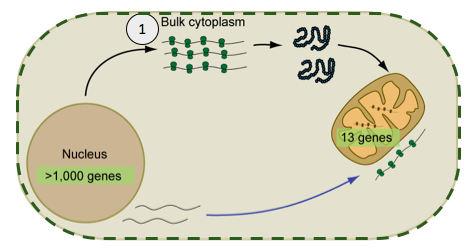
\includegraphics[width=55mm,height=35mm]{Figures/bulk.png} &
		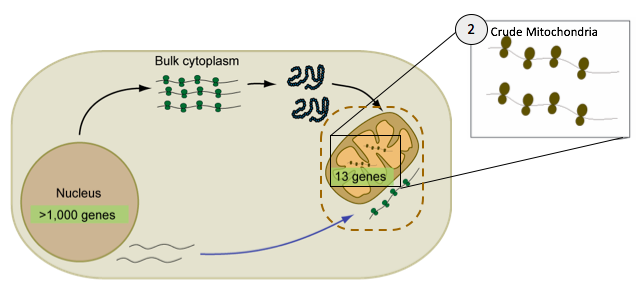
\includegraphics[width=85mm,height=55mm]{Figures/crude_mitochondria.png} \\
		Bulk Cytoplasm & Crude Mitochondria
	\end{tabular}
	\caption{Datasets}
	\label{fig: Datasets}
\end{figure}
By studying genes from these two different pools, we hope to understand the translational coordination between the nuclear and mitochondrial genomes during mitochondrial biogenesis. Specifically, the data will be in the form of expression values (numeric) of each gene at different time points.

\subsection{Clustering Gene Expression Values}
\textit{Clustering} is an exploratory data analysis technique that allows us to organize a pile of information into meaningful subgroups (\textit{clusters}) without having any prior knowledge of their group memberships. Each cluster that may arise during the analysis defines a group of objects that share a certain degree of similarity but are more dissimilar to objects in other clusters, which is why clustering is also sometimes called 'unsupervised classification'.

Clustering has many applications to computational biology. For example, we consider expression profiles of many genes taken at various developmental stages. Clustering may show that certain sets of genes line up (i.e. show the same expression levels) at various stages. This may indicate that this set of gene has common expression or regulation and we can use this to infer similar function. Furthermore, if we find a uncharacterised gene in such a set of genes, we can reason that the uncharacterised genes also has a similar function through guilt by association. 

For this project, we apply this principle which means we are working with the common assumption that genes with similar biological properties will fall under the same cluster in terms of their expression values \cite{Eisen14863}. Thus, we hope that after getting different clusters or groups of genes, each cluster may exhibit similar biological properties and distinct biological properties from one another. Afterwards, we will then be able to provide an additional information to what kind of communication or mechanism that occurs between nuclear and mitochondrial genomes.

%----------------------------------------------------------------------------------------

\section{Literature Review}
Time-series expression experiments are used to study a wide range of biological systems. More than $80\%$ of all time series expression datasets are short ($8$ time points or fewer). These dataset present unique challenges. On account of the large number of genes profiled (often tens of thousands) and the small number of time points many patterns are expected to arise at random. Most clustering algorithms are unable to distinguish between real and random patterns \cite{Ernst2005}.

Clustering algorithms have been extensively applied in the study of time-series gene expression data. Hierarchical clustering \cite{Eisen14863} and other standard clustering methods such as K-means \cite{Duda73a} are often used for this task. Furthermore, time-series data by nature or structure tends to be correlated, which can normally be dealt with the use of multivariate Gaussian mixture model \cite{Eirola}. Although these clustering algorithms have yielded many biological insights, they are not designed for time-series data, especially for short time-series. Specifically, all these methods assume that data at each time point are collected independent of each other, ignoring the sequential nature of time-series data. 

Some algorithms have been specifically modified or created to handle time-series biological data. These algorithms include clustering based on the dynamics of the expression patterns \cite{Ramoni9121}, clustering using the continuous representation of the profile \cite{Bar-Joseph} and clustering using a Hidden Markov Model (HMM) \cite{Rabiner1989, Schliep2003}. Spectral clustering \cite{Wang} has also been developed to deal with time-series data. Nonetheless, there has not been many studies done for spectral clustering and it remains an unpopular clustering algorithm for time-series data.

Furthermore, mixed-effect models or fitting cubic splines \cite{Ma2006, Golumbeanu2017, Zhang2014} to time-series expression values, which are similar to mixture model and Bayesian approach to mixture model \cite{Jia2008} have also been developed to improve the clustering of time-series data. While these algorithms work well for relatively long series dataset (10 time points or more), they are not appropriate for short time-series \cite{Ernst2005}. On account of the noise and the small number of points for each gene, most clustering algorithms cannot distinguish between patterns that occur because of random chance and clusters that represent a real response to the biological experiment. Short Time-series Expression Miner (STEM) \cite{Ernst2005} is one commonly used algorithm to deal with this problem due to the way it is constructed and its success in producing biologically significant clusters.

Nevertheless, the study of clustering algorithm for time-series data is still inconclusive which means that it may still ultimately depend on the nature of the data itself. For instance, hierarchical clustering remains a popular choice for clustering gene time-series expression values despite its failure for some cases. Hence, other than applying STEM in our report, we will still study popular clustering algorithms such as Gaussian Mixture Model, K-means and Hierarchical Clustering. 
% Chapter 3

\chapter{Theories and Tools Used}
This chapter will cover some theories and tools used in the various machine learning algorithms and our analysis.
\setlength{\belowdisplayskip}{1pt} \setlength{\belowdisplayshortskip}{1pt}
\setlength{\abovedisplayskip}{1pt} \setlength{\abovedisplayshortskip}{1pt}

\section{Expectation Maximisation (EM) Algorithm} \label{2.1}
EM is an iterative method that attempts to find the maximum likelihood estimator of a parameter $\theta$ of a parametric probability distribution \cite{Gupta}. As a general procedure, EM is used to estimate parameters for probabilistic models with hidden or latent variables. EM algorithm is used both in Gaussian Mixture Model (refer to Chapter \ref{3.2}) and K-means (will not be covered in this report). 
\subsection{Outline}
Consider a probabilistic model in which we have: observed data $y$, a parametric density $p(y|\theta)$, a description of some complete data $x$ that we wish we had, and the parametric density $p(x|\theta)$. We assume that the complete data can be modelled as a continuous random vector $X$ with density $p(x|\theta)$, where $\theta \in \omega$ for some set $\omega$. We do not observe $X$ directly; instead, we observe a realization $y$ of the random vector $Y$ that depends on $X$. 

Given that we only have $y$, we want to find the maximum likelihood estimate (MLE) of $\theta$:
\begin{equation*}
\theta_{\text{MLE}} = \operatorname{arg\,max}_{\theta \in \omega} \log p(y|\theta)
\end{equation*}
However, for some problem it is difficult to solve the above optimization problem and here where EM comes to help. We make a guess about the complete data $X$ and solve for the $\theta$ that maximizes the (expected) log-likelihood of $X$. And once we have an estimate for $\theta$, we can make a better guess about the complete data $X$, and iterate. Here are the steps in summary:
\begin{itemize}
	\item Let $m=0$ and make an initial estimate $\theta^{(m)}=\theta$.
	\item Given the observed data $y$ and pretending for the moment that our current guess $\theta^{(m)}$ is correct, formulate the conditional probability distribution $p(x|y, \theta^{(m)})$ for the complete data $x$.
	\item Using the conditional probability distribution $p(x|y, \theta^{(m)})$ calculated in Step 2, form the \textit{conditional expected log-likelihood}, which is called the $Q$-function:
	\begin{equation*}
	Q(\theta|\theta^{(m)}) = \int_{\omega (y)} \log p(x|\theta)p(x|y, \theta^{(m)})dx = \mathbb{E}_{X|y,\theta^{(m)}} \log p(X|\theta)
	\end{equation*}
	\item Find the $\theta$ that maximizes the $Q$-function; the result is our new estimate $\theta^{(m+1)}$.
	\item Let $m:=m+1$ and go back to Step 2. The EM algorithm does not specify stopping criterion; standard criterion is to iterate until the estimate stops changing: $||\theta^{(m+1)}-\theta^{(m)}|| < \epsilon$ for some $\epsilon>0$, or to iterate until the log-likelihood $l(\theta) = \log p(y|\theta)$ stops changing: $|l(\theta^{(m+1)})-l(\theta^{(m)})|<\epsilon$ for some $\epsilon>0$.
\end{itemize}

The monotonicity of the EM algorithm guarantees that as EM iterates, its guesses will not get worse in terms of their likelihood (the proof can be referred to \cite{Bishop2013}), but the monotonicity alone cannot guarantee the convergence of the sequence $\{\theta^{(m)}\}$. Hence, in practice, we perform EM algorithm multiple times to get the best fit. 
%----------------------------------------------------------------------------------------

\section{Determining Optimal Number of Clusters} \label{2.2}
Here we describe a method to determine the optimal number of clusters for Gaussian Mixture Model.
\subsection{BIC and AIC} \label{2.2.1}
%Akaike, H.: A new look at the statistical model identification
%Schwarz, G.: Estimating the dimension of a model
%GMM for Time Series Modelling, Forecasting and Interpolation
When we want to find optimal number of clusters from various clustering algorithms, too few components are not able to model the distribution appropriately, while having too many components cause issues of overfitting. The number of components can be selected according to Akaike Information Criterion (AIC) \cite{Akaike1998} or the Bayesian Information Criterion (BIC) \cite{Schwarz1978}. 
\subsubsection{Outline}
BIC and AIC impose a penalty on the total number of parameters, scaled by the logarithm of sample size, so as to strike a balance between the goodness-of-fit and the model complexity.
Both are expressed as a function of the log-likelihood of the converged mixture model:
\begin{align*}
AIC  &= -2\log L(\theta) + 2P\\
BIC &= -2\log L(\theta) + \log(N)P
\end{align*}
where $P$ is the number of free parameters and $N$ is the number of data points. The clustering algorithm (Mixture Model in our case) is run for several different values of $K$, and the model which minimises the chosen criterion is selected. As $\log(N)>2$ in most cases, BIC more aggresively penalises an increase in $P$, generally resulting in a smaller choice for $K$ than by AIC. Lower AIC or BIC values indicates better fitting models. We should also ensure that our choices for $k$ and the covariance matrix structure is appropriate for our application. 

\subsection{Elbow Method Analysis} \label{2.2.2}
For \textit{k-means}, since we do not know the definitive answer on the optimal number of clusters, we need a method to quantify the quality of clustering. \textit{Elbow Method} is a graphical tool that helps us to estimate the optimal number of cluster $k$ for our task. 
\subsubsection{Outline}
The elbow method plots the value of the cost function produced by different values of $k$. This is motivated by the use of intrinsic metrics - such as the within-cluster sum-of-squared-error (distortion). Intuitively, we can say that, if $k$ increases, the distortion will decrease; each cluster will have fewer constituent instances, and the instances will be closer to their respective centroids. However, the improvements to the average distortion will decline as $k$ increases. The value of $k$ at which the improvement to the distortion declines the most is called the elbow (Figure \ref{fig: elbow}). Here is the method in summary:
\begin{itemize}
	\item Find the sum of intra-cluster distances between points $\in D_k$ in a given cluster $C_k$, \\$C_k=\sum\limits_{x_i \in D_k}\sum\limits_{x_j \in D_k} \lVert x_i-x_j \rVert ^2 = 2n_k \sum\limits_{x_i \in D_k} = \lVert x_i - \mu _k \rVert ^2$
	\item Find the normalized intra-cluster sums of squares: measure compactness of our clustering, $W_k = \sum\limits_{k=1}^K \frac{1}{2n_k}C_k$
	\item Look at the $\%$ of variance explained as a function of the number of clusters
\end{itemize}

\begin{figure}[h] 
	\centering
	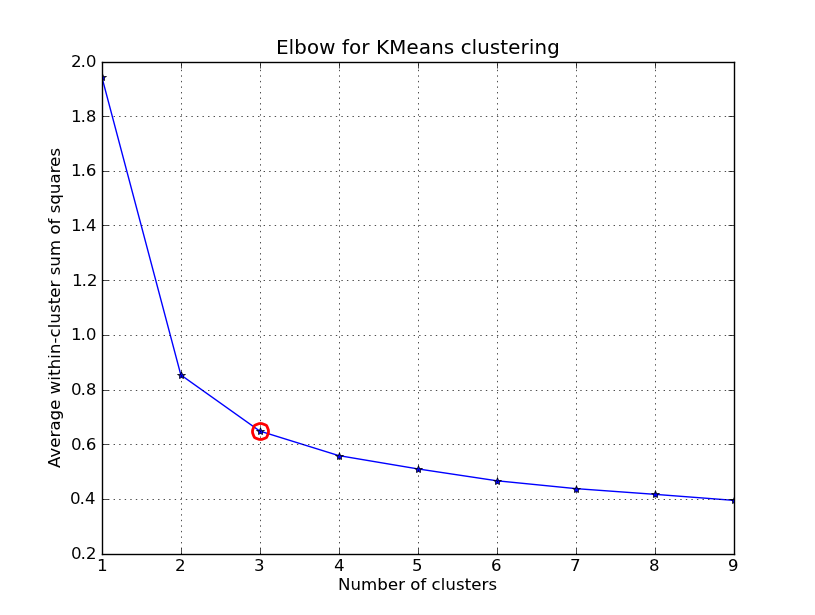
\includegraphics[scale= 0.5]{Figures/elbow_curve_expected.png}
	\caption{Ideal elbow curve where it easy to identify the 'elbow' (red circle)}
	\label{fig: elbow}
\end{figure}

\subsection{Gap Statistic} \label{2.2.3}
Gap Statistic \cite{Tibshirani2001} is another popular method used to determine the optimal number of clusters from various clustering algorithms such as \textit{k-means}. 
\subsubsection{Outline}
Given our data $\{x_{ij}\}, i =1,2,\dots,n, j = 1,2,\dots, p$, consist of $p$ features measured on $n$ independent observations. Let $d_{ii'}$ denote the distance between observations $i$ and $i'$. For simplicity, we use euclidean distance $d_{ii'} = \sum_j (x_{ij}-x_{i'j})^2$.
Suppose that we have clustered the data into $k$ clusters $C_1, C_2, \dots, C_k$, with $C_r$ denoting the indices of observations in cluster $r$, and $n_r = |C_r|$. Let $D_k$ and $W_k$ be the same as that in elbow curve analysis. Then, the idea of gap statistic analysis is to standardize the graph of $\log(W_k)$ by comparing it with its expectation under an appropriate null reference distribution of the data. Our estimate of the optimal number of clusters is the the value of $k$ for which $\log(W_k)$ falls the farthest below this reference curve. Hence, we define $Gap_n(k) = E_n^*\{\log W_k\}-\log W_k$ where $E_n^*$ denotes the expectation under a sample of size $n$ from the reference distribution. Our estimate $k^*$ will be the value maximizing $Gap_n(k)$ after we take the sampling distribution into account. Note that this estimate is very general, applicable to any clustering method and distance measure $d_{ii'}$. Here is the method in summary:
\begin{itemize}
	\item Compare $\log W_k$ vs null reference distribution of the data, i.e. a distribution with no obvious clustering.
	\item Find optimal $K: \operatorname*{arg\,max}\limits_k Gap_n(k) = E_n^*\{\log W_k\}-\log W_k$
	\item OR Estimate $E_n^*\{\log W_k\} = \frac{1}{B}\sum\limits_{b=1}^B \log (W_{kb}^*)$, each of which is computed from a Monte Carlo sample $X_1^*,\cdots, X_n^*$ drawn from our reference distribution.
	\item Then, Simulation error, $s_k = sd(k)\sqrt{1+\frac{1}{B}}$, where $sd(k)^2=\frac{1}{B}\sum\limits_b(\log W_{kb}^*-\frac{1}{B}\sum\limits_{b=1}^B \log(W_{kb}^*))^2$
	\item Find optimal $k^*: \operatorname*{arg\,min}\limits_k Gap(k)\geq Gap(k+1)-s_{k+1}$. This is a more refined approach for better control of the rejection of the null model.
\end{itemize}

%----------------------------------------------------------------------------------------

\section{Performance Measures} \label{2.3}
After we have found the optimal number of clusters for our data, we need to evaluate the quality of our clustering. In our project, we have a benchmark algorithm (see \ref{3.1}) which will be covered in the next chapter. We assume that this algorithm will yield the most optimal clustering. Then, we want to compare other clustering algorithms to this benchmark algorithm. There are two measures that we use for this project: 
\subsection{Clustering Accuracy (CA)} \label{2.3.1}
Let $\{t_i\}$ denote the true classes and $\{c_j\}$ denote the clusters found by a cluster algorithm. We then label all the data in cluster $c_j$ as $t_i$ if they share the most data objects. Note that the number of clusters need not be the same as the number of classes. Then we can calculate the clustering accuracy \cite{Wang}, $\eta$ as:
\begin{equation*}
\eta = \frac{\sum_x I(c_i(x) = t_j(x))}{M}
\end{equation*}
where $I(.)$ is the indicator function, $c_i(x)$ is the label of the cluster which $x$ belongs to, $t_j(x)$ is the true class of $x$, and $M$ is the size of the dataset. The closer the value to $1$, the better the clustering is, and the closer it is to $0$, the worse the clustering is.

\subsection{ME Distance} \label{2.3.2}
This method which is first introduced in \cite{Meila} also computes how far the clusters obtained from any clustering algorithm are from the \textit{true} clusters. 
\subsubsection{Definition}
A \textit{clustering} $C$ of a finite dataset, assumed w.l.o.g to be $\{1,2,\dots,n\} = [n]$, is a partition of the dataset into disjoint, non-empty subsets called \textit{clusters}. If the partition has $K$ clusters, we write $C=\{C_1,C_2,\dots,C_k\}$ and denote by $n_k= |C_k|, \sum_k n_k = n$. A clustering can be represented by a $n \times K$ matrix $\tilde{X}$, whose columns represent the indicator vectors of the $K$ clusters. 
\begin{equation*}
\tilde{X}_{ik} = \begin{cases}
1 & \text{if $i \in C_k$} \\
0 & \text{otherwise}
\end{cases}
\end{equation*}

The columns of $\tilde{X}'$ are mutually orthogonal vectors. If we normalize these to length 1, we obtained \textit{normalized} representation $X$.
\begin{equation*}
X_{ik} = \begin{cases}
n_k^{-1/2} & \text{if $i \in C_k$} \\
0 & \text{otherwise}
\end{cases}
\end{equation*}

\subsubsection{The Misclassification Error (ME) Distance between Clusterings}
The \textit{confusion matrix} of two clusterings $C = \{C_1,C_2, \dots, C_K\}$ and $C' = \{C'_1, C'_2, \dots, C'_{K'}\}$ is defined as the $K \times K'$ matrix $M = [m_{kk'}]$ with $m_{kk'}= |C_k \cap C'_k|$. A distance between two clusterings is typically a permutation invariant function of the confusion matrix $M$. We will assume $K= K'$ for simplicity. The \textit{Misclassification Error (ME)} distance is defined as 
\begin{equation*}
d(\tilde{X}, \tilde{X}') = 1 - \frac{1}{n}\operatorname{max}_{\pi \in \prod_K}\sum_k m_{k,\pi(k)}
\end{equation*}
The distance represents the well known cost of classification, minimized over all permutations of the labels $[K]$. $d$ can be computed in polynomial time by a maximum bipartite matching algorithm \cite{Papadimitriou}. Unlike \textit{CA}, we want \textit{ME} distance as close as possible to $1$.
%----------------------------------------------------------------------------------------
\section{Gene Ontology (GO)} \label{2.4}
Ultimately, we want to conclude that each cluster obtained from the algorithm contains genes that will share similar biological properties and distinct biological properties with another cluster. We then apply GO analysis on all the different clusters. Ontology on itself means a representation of something we know about. GO then provides an ontology of defined terms representing gene product properties. Each GO term within the ontology has a term name, which may be a word or string of words; a unique alphanumeric identifier; a definition with cited sources; and a name-space indicating the domain to which it belongs. The ontology covers:

\begin{itemize}
	\item \textbf{cellular component}: the parts of a cell or its extracellular environment;
	\item \textbf{molecular function}: the elemental activities of a gene product at the molecular level, such as binding or catalysis;
	\item \textbf{biological process}: operations or sets of molecular events with a defined beginning and end, pertinent to the functioning of integrated living units: cells, tissues, organs, and organisms.
\end{itemize}

Another category that we will be looking at is KEGG pathway, which tells us a different pathway maps representing our knowledge on the molecular interaction, reaction and relation networks for various biological processes. For this project, we particularly are interested in pathway such as Oxidative Phosphorilation (refer to \ref{Objective}). GO helps to perform enrichment analysis on gene sets. For example, given a set of genes that are up-regulated under certain conditions, an enrichment analysis will find which GO terms are over-represented (or under-represented) using annotations for that gene set (Figure \ref{fig: GO}). The results will tell us lists of significant shared GO terms used to describe the set of genes that users entered and \textit{p-value}.

\begin{figure}[h!]
	\centering
	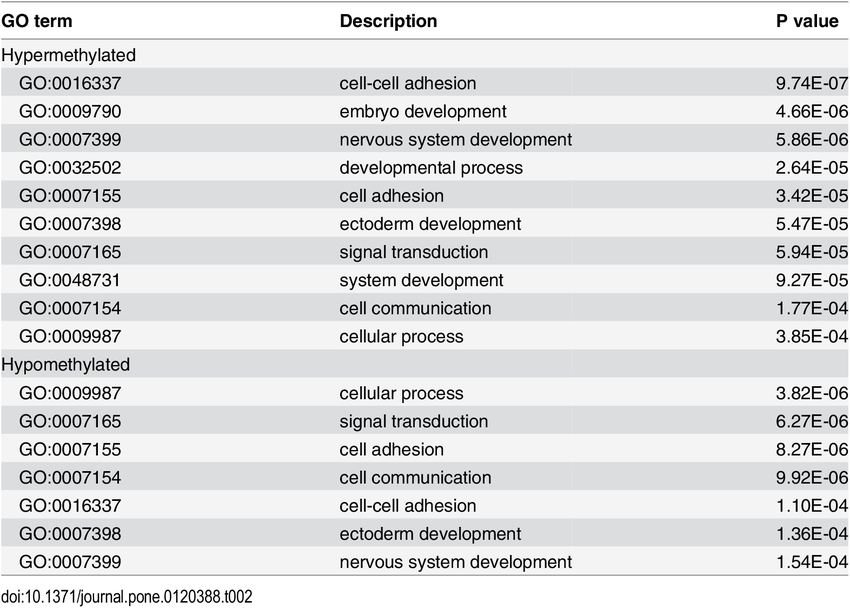
\includegraphics[width=100mm,height=70mm ]{Figures/sample_go.png}
	\caption{Sample GO}
	\label{fig: GO}
\end{figure}

\textit{p-value} here tells us the probability of seeing at least $x$ number of genes out of the total $n$ genes in the list annotated to a particular GO term, given the proportion of genes in the whole genome that are annotated to that GO term. That is, the GO terms shared by the genes in the user's list are compared to the background distribution of annotation. The smaller the \textit{p-value} is, the more significant the particular GO term associated with the group of genes is (i.e. the less likely the observed annotation of the particular GO term to a group of genes occurs by chance).  In other words, when searching the process ontology, if all of the genes in a group were associated with "DNA repair", this term would be significant.

%----------------------------------------------------------------------------------------
% Chapter 4

\chapter{Algorithms}
\setlength{\belowdisplayskip}{1pt} \setlength{\belowdisplayshortskip}{1pt}
\setlength{\abovedisplayskip}{1pt} \setlength{\abovedisplayshortskip}{1pt}
\section{Short Time-series Expression Miner (STEM)} \label{3.1}
This clustering algorithm has been specifically designed to address the problems with short time-series data of gene expression values \cite{Ernst2005}. STEM works by assigning genes to a predefined set of model profiles that capture the potential distinct patterns that can be expected from the experiment. It then filters out profiles that are not significant which allows us to obtain the optimal number of clusters. Additionally, it is able to capture the time dependencies of the data. As such, we decided to pick this as our benchmark algorithm. Lastly, the clustering results are verified with GO analysis. 

\subsection{Outline}
The following step-by-step list summarizes the STEM algorithm:
	\begin{itemize}
		\item Generate all possible model profiles whereby a user needs to select parameter $c$ to determine the maximum unit of change between time points.
		\item Select parameter $m$, the number of distinct model profiles.
		\item Assign genes to the model profiles obtained previously.
		\item Determine statistical significance of each of these profiles using \textit{Permutation Test}. Keep the significant profiles.
		\item Select parameter $\delta$, threshold distance between profiles to group similar significant profiles
	\end{itemize}
This algorithm generates profiles that are actually independent of the data which can be good or bad depending on the data itself. Nevertheless, Friedman \cite{Sivriver2011} argues that this actually reduces the performance of this algorithm. In short, STEM helps in enumerating distinct model profiles that are representative of any expression profile we would probably see.

\subsection{Generating Model Profiles}
The algorithm requires conversion of the raw expression values into log ratios where the ratios are with respect to the expression of the first time point. This means at $t_0$, all values will be zero. We then define parameter $c$ as the maximum amount of change a gene can have between successive time points. If $x_t$ is the expression value of a gene at time point $t$, then $x_{t+1}$ can take integer values in $[x_t -c, x_t+c]$. For example, when $c=2$, a gene can go down either one or two units, remain constant, or go up one or two units. 

The number of all possible model profiles will be $|P| = (2c+1)^{n-1}$, where $n$ is the number of time points in a profile ($7$ for our data) and $P$ is the set of all possible profiles. As we observe, the number of profiles grows as a high order polynomial in $c$. For example, with $n=6$ and $c=3, |P| = 16807$. While, the number goes down to only $3125$ when we choose $c=2$. 

\subsubsection{Selecting Distinct Model Profiles}
Our aim is to select a set of model profiles all of which are distinct from one another, but representative of any expression profile we would probably see. Hence, we want to ensure that the resulting clusters would not be very small. This is done by selecting a set $R \subset P$ with $|R|=m$ such that the minimum distance between any two profiles in $R$ is maximized. Mathematically, this is equivalent to 
\begin{equation} \label{eq:1}
\operatorname*{arg\,max}_{R \subset P, |R|=m} \operatorname*{arg\, min}_{p_1,p_2 \in R} d(p_1,p_2)
\end{equation} where $d$ is a distance metric.

\subsubsection{Distance Measure}
STEM uses \textbf{correlation coefficient} $\rho(x,y)$ as the distance measures as it has been yielding positive results in computational biology, especially when used for clustering \cite{Eisen14863}. More specifically, STEM uses $gm(x,y) = 1- \rho (x,y)$ as $\rho(x,y)$ can be negative and does not satisfy the triangle inequality and hence is not a metric.

Even though, $gm(x,y)$ is still not a metric since it also does not satisfy the triangle inequality, it satisfies a generalized version of the triangle inequality. This inequality actually also proves that the correlation coefficient is a transitive measure, which means when using it, two highly dissimilar profiles cannot be very similar to a third profile.
\begin{align*}
gm(x,z) \leq 2(gm(x,y) + gm(y,z))
\end{align*}
%read more on the supporting website

For a set $R$ let $b(R) = \operatorname{min}_{p_1,p_2\in R}d(p_1,p_2)$, i.e. $b(R)$ is the minimum distance between model profiles in R, which is the quantity we want to maximize. Let $R'$ be the set of profiles that maximizes equation \ref{eq:1}. Thus, $b(R')$ is the optimal value we can achieve. Unfortunately, this is a NP-hard problem. Moreover, an approximation that guarantees that a solution that is better than $\frac{b(R')}{2}$ is also NP-hard. Here, STEM uses a greedy algorithm that is guaranteed to find such a set, i.e. algorithm finds a set of profiles $R$, with $b(R) \geq \frac{b(R')}{2}$.
\begin{table}[H]
		\renewcommand{\arraystretch}{0.5}
	{\LinesNumberedHidden
		\begin{algorithm}[H]
			\SetKwInOut{Input}{Input}
			\SetKwInOut{Output}{Output}
			 Let $p_1 \in P$ be the profile that always goes down $1$ unit between time points
			\begin{enumerate}
				\item $R \leftarrow \{p_1\}$; $L \leftarrow P \textbackslash \{p_1\}$
				\item for $i \leftarrow 2$ to $m$ do 
				\item let $p \in L$ where $p = \operatorname*{arg\,max}_{p_1 \in R}d(p,p_1)$
						\item $R \leftarrow R\cup \{p\}; L \leftarrow L \textbackslash \{p\}$ 
				\item return $R$								
			\end{enumerate}
\caption{Select Distinct Profiles $(d,P,m)$}
	\end{algorithm}}
\caption{Greedy Approximation Algorithm to choose a set of $m$ distinct profiles}
\label{algo: Greedy Algorithm}
\end{table}
The following theorem (proof found here \cite{Ernst2005}) proves the optimality of this algorithm:
\begin{theorem}
	Let $d$ be a distance metric. Let $R' \subset P$ be the set of profiles that maximizes \ref{eq:1}. Let $R \subset P$ be the set of profiles returned by the \autoref{algo: Greedy Algorithm}, then $b(R) \geq \frac{b(R')}{2}$.
\end{theorem}

\subsection{Finding Significant Model Profiles}
This step will return different profiles together with the genes assigned to them. Furthermore, this step also tells us the \textit{p-value} of the model profiles, where a small value means that the number of data profiles belonging to the cluster represented by the model profile is significantly large. This involves two steps: assigning the genes according to their expression values to the different model profiles generated earlier and performing \textit{Permutation Test} to identify significant model profiles.

\subsubsection{Assigning Genes to Model Profiles}
Given a set $M$ of model profiles and a set of genes $G$, each gene $g \in G$ is assigned to a model expression profile $m_i \in M$ such that $d(e_g, m_i)$ is the minimum over all $m_i \in M$, where $e_g$ is the temporal expression profile for gene $g$. If the above distance is minimized by $h>1$ model profiles (i.e. we have ties) then we assign $g$ to all of these profiles, but weigh the assignment in the counts as $\frac{1}{h}$. We count the number of genes assigned to each model profile and denote this number for profile $m_i$ by $t(m_i)$.

\subsubsection{Permutation Test}
We perform \textit{Permutation Test} to identify model profiles that are significantly enriched for genes in our experiment. The null hypothesis will be that the data are memoryless, i.e. the probability of observing a value at any time point is independent of past and future values. Hence, under $H_0$, any profile we observe is a result of random fluctuation in the measured values for genes assigned to that profile. Model profiles that represent true biological function deviate significantly from $H_0$ since many more genes than expected by random chance are assigned to them. \textit{Permutation Test} is used here to quantify the expected number of genes that would have been assigned to each model profile if the data were generated at random. 

For each possible permutation we assign genes to their closest model profile. If we let $s_i^j$ be the number of genes assigned to model profile $i = 1,\cdots,m$ in permutation $j=1,\cdots,n!$, then $E_i = \frac{\sum_j s_i^j}{n!}$ is the expected number of profiles assigned to the cluster, when considering a random permutation.

Since each gene is assigned to one of the profiles, we can assume that the number of genes, $N$ in each profile $\sim \text{Bin}(|G|,E_i/|G|)$. Thus, the algorithm computes the \textit{p-value}$= P(N \geq t(m_i))$ of seeing $t(m_i)$ genes assigned to profile $p_i$. Moreover, we need to apply Bonferroni corrections as we are testing more than one model expression profile. Thus, the critical region will be $P(N \geq t(m_i)) \le \frac{\alpha}{m}$ for $\alpha \%$ level of significance.

\subsection{Grouping Significant Profiles}

The idea of grouping significant profiles is motivated by noise. Due to noise, it is impossible to rule out close profiles (even if not the closest) as being the true profile for individual genes. Then, the logical and natural step is to split the set of significant profiles into groups of similar profiles. If we have a measurement of the noise (e.g. from repeat experiments) it is possible to determine a distance threshold $\delta$ below which two profiles are considered similar (the difference between genes assigned to these two may be attributed to noise). Such model profiles represent similar enough expression patterns and thus should be grouped together.

We transform this problem of grouping significant profiles into a graph theoretical problem. Define the graph $G(V,E)$ where $V$ is the set of significant model profiles and $E$ the set of edges. Two profiles $v_1,v_2 \in V$ are connected with an edge iff $d(v_1,v_2) \leq \delta$. Cliques in this graph correspond to sets of significant profiles which are all similar to one another. Here we are interested in identifying large cliques of profiles which are all very similar to each other. This naturally leads to a greedy algorithm to partition the graph into cliques and thus to group significant profiles.

In summary, the greedy algorithm grows a cluster $C_i$ around each statistically significant profile $p_i$. Initially, $C_i = \{p_i\}$. Next, we look for a profile $p_j$ such that $p_j$ is the closest profile to $p_i$ that is not already included in $C_i$. If $d(p_j,p_k) \leq \delta$ for all profiles $p_k \in C_i$, we add $p_j$ to $C_i$ and repeat this process, otherwise we stop and declare $C_i$ as the cluster for $p_i$. After a temporary group has been built for each profile, a final grouping is formed by selecting the largest temporary groups one by one. Since each significant profile must reside in a single final group, the profiles that belong to a selected group are removed from every other temporary group. A new group is added to the list of final groups until there are no profiles left to be grouped. 

\subsection{Challenges}
Since the set of potential profiles are not selected from the data, they might contain profiles that do not represent true biological responses. An additional obstacle is that the clustering is done on the noisy and missing expression patterns of genes which might lead to false assignments to clusters \cite{Sivriver2011}.

Furthermore, identifying groups of similar model profiles seems like a good idea, yet there are some problems. Aforementioned above, it is not trivial to assign a meaningful value to $\delta$. In the biological results of \cite{Ernst2005}, a value of $\delta =0.3$ is used. 

The grouping of model profiles also complicates the analysis of the clustering results, or at least raises some questions. Should the results of the grouping be integrated into the clustering of the data profiles by combining the clusters that belong to the same group, or would some kind of separate treatment of the grouping results be more appropriate?
%----------------------------------------------------------------------------------------

\section{Mixture Model} \label{3.2}
In this model \cite{Bishop2013}, we are assuming that our data are generated i.i.d. by a mixture of $k$ Gaussians, and we want to estimate the mean and covariances of the $k$ Gaussians. Yet, we do not know which of the observed points came from which Gaussian. Our goal is to estimate the $k$ means and $k$ covariances, and $k$ weights that specify how likely each Gaussian is to be chosen; this entire set of parameters is $\theta$. 
\subsection{Outline}
Given $n$ i.i.d. samples $y_1, y_2, \dots, y_n \in \mathbb{R}^d$ drawn from a GMM with $k$ components, the goal is to estimate the parameter set $\theta = \{(w_j, \mu_j, \Sigma_k)\}_{j=1}^k$. 
The GMM has density 
\begin{equation*}
p(Y_i = y_i | \theta) = \sum_{j=1}^k w_j N(y_i|\mu_j, \Sigma_j), w_j>0, \sum_{j=1}^k w_j = 1
\end{equation*}

Let $\gamma_{ij}^{(m)}$ be the estimate at the $m$th iteration of the probability that the $i$th sample was generated by the $j$th Gaussian component, that is, 
\begin{equation*}
\gamma_{ij}^{(m)} = P(Z_i=j|y_i, \theta^{(m)}) = \frac{w_j^{(m)}N(y_i|\mu_j, \Sigma_j)}{\sum_{l=1}^kw_l^{(m)}N(y_i|\mu_l, \Sigma_l)}
\end{equation*}
which satisfies $\sum_{j=1}^k \gamma_{ij}^{(m)}=1.$

We summarize the whole algorithm in \autoref{algo: EM algorithm for GMM} below.
\begin{table}[H]
	{\LinesNumberedHidden
		\begin{algorithm}[H]
			\SetKwInOut{Input}{Input}
			\SetKwInOut{Output}{Output}
			%\SetAlgorithmName{Algorithm}{}
			\begin{enumerate}
				\item Initialization: Choose initial estimates $w_j^{(0)}, \mu_j^{(0)}, \Sigma_j^{(0)}, j =1, \dots, k$, and compute the initial log-likelihood,
				$l^{(0)} = \frac{1}{n}\sum_{i=1}^n \log(\sum_{j=1}^kw_j^{(0)}N(y_i|\mu_j^{(0)},\Sigma_j^{(0)})).$
				\item \textbf{E-step} For $j = 1,\dots,k$, compute
				$\gamma_{ij}^{(m)} = P(Z_i=j|y_i, \theta^{(m)}) = \frac{w_j^{(m)}N(y_i|\mu_j, \Sigma_j)}{\sum_{l=1}^kw_l^{(m)}N(y_i|\mu_l, \Sigma_l)}, i = 1, \dots, n, $
				and $n_j^{(m)} = \sum_{i=1}^n \gamma_{ij}^{(m)}$
				\item \textbf{M-step} For $j = 1,\dots, k$, compute the new estimation
				$$w_j^{(m+1)} = \frac{n_j^{(m)}}{n}, \mu_j^{(m+1)} = \frac{1}{n^{(m)}}\sum_{i=1}^n\gamma_{ij}^{(m)}y_i,$$
				$$\Sigma_j^{(m+1)} = \frac{1}{n_j^{(m)}}\sum_{i=1}^n \gamma_{ij}^{(m)}(y_i-\mu_j^{(m+1)})(y_i-\mu_j^{(m+1)})^T,$$
				\item Convergence check: Compute the new log-likelihood $l^{(m+1)} = \frac{1}{n}\sum_{i=1}^n \log(\sum_{j=1}^kw_j^{(m+1)}N(y_i|\mu_j^{(m+1)}, \Sigma_j^{(m+1)}))$. \\
				Return to Step 2 if $|l^{(m+1)}-l^{(m)}| > \epsilon$ for a present threshold $\epsilon$, otherwise end.
			\end{enumerate}
			\caption{EM for GMM}
	\end{algorithm}}
	\caption{Summary of EM Algorithm for GMM}
	\label{algo: EM algorithm for GMM}
\end{table}
As the algorithm tends to occasionally converge to sub-optimal solutions, the procedure can be repeated to find the best fit. This model also allows for different types of covariance matrices for each mixture component, which is summarized at Table \ref{Tab: Different Covariance Matrices} below. For this report, we only consider the two simple cases: Diagonal and Spherical.
\begin{table}[h]
	\centering
	\begin{tabular}{|l|l|l|ll}
		\cline{1-3}
		\textbf{Covariance} & \textbf{Description}                                                                                                      & \textbf{\# parameters} &                       &                       \\ \cline{1-3} \cline{5-5} 
		Full                & \begin{tabular}[c]{@{}l@{}}Each component has its own general covariance matrix\\ (correlated predictors)\end{tabular}    & $kd(d+1)/2$           & \multicolumn{1}{l|}{} & \multicolumn{1}{l|}{} \\ \cline{1-3} \cline{5-5} 
		Tied                & All components share the same general covariance matrix                                                                   & $d(d+1)/2$             &                       &                       \\ \cline{1-3}
		Diagonal            & \begin{tabular}[c]{@{}l@{}}Each component has its own diagonal covariance matrix\\ (uncorrelated predictors)\end{tabular} & $kd$                   &                       &                       \\ \cline{1-3}
		Spherical           & Each component has its own single variance                                                                                & $k$                    &                       &                       \\ \cline{1-3}
	\end{tabular}
	\caption{DIfferent Covariance Matrices} \label{Tab: Different Covariance Matrices}
\end{table}
%----------------------------------------------------------------------------------------
\section{K-means} \label{3.3}
This searches for a specific number of clusters $k$ maximizing a global target function \cite{Bishop2013}. Clusters are defined by their center. Iteratively, genes are assigned to the best-matching cluster and then the clusters' center values are updated. In our context and other real-world applications in general, we do not have any ground truth category information about our data. Thus, our goal is to group the samples based on their feature similarities (euclidean distance in this case), which can be achieved using the k-means algorithm that can be summarized by the following four steps (Figure \ref{fig: kmeans}):
\begin{itemize}
	\item Randomly pick $k$ centroids from the sample points as initial cluster centers.
	\item Assign each sample to the nearest centroid $\mu^{(j)}, j \in \{1,\dots,k\}$
	\item Move the centroids to the center of the samples that were assigned to it.
	\item Repeat steps 2 and 3 until the cluster assignments do not change or a user-defined tolerance of a maximum number of iterations is reached.
\end{itemize}

\begin{figure}[h] 
	\centering
	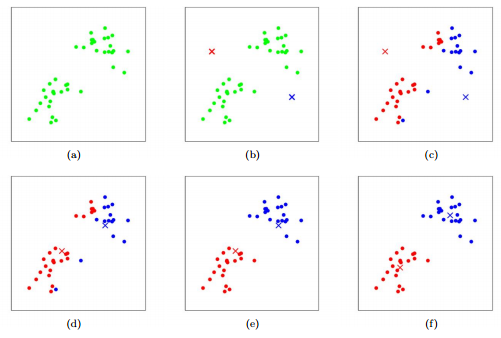
\includegraphics[scale = 0.8]{Figures/kmeans.png}
	\caption{Iterative steps for k-means}
	\label{fig: kmeans}
\end{figure}

\subsection{Outline}
Mathematically, the steps above can be written as:
Given a dataset $D = \bigl\{x_t\bigr\}^n_{t=1}$ and fix a number of clusters $1 \leq k \leq n$, we want to minimize the cost function 
\begin{equation*}
J = \sum_{j=1}^k \sum_{x \in D_j} \lVert x-\mu_j \rVert ^2
\end{equation*}
This cost function is the \textit{similarity measure} between our data. 
$D$ is partitioned into $D_1, D_2, \cdots, D_k$

\begin{itemize}
	\item Step 0 Initialize the centroids $\mu_{j}^{(1)}, j = 1,\cdots,k$ randomly 
	
	\item Step $l \in \mathbb{N}$ (E-step) Assign each point $x_t$ to its closest centroid, \begin{equation}\label{eq:3.1}
	j_t = \operatorname*{arg\,min}_{j=1,\cdots,k} \lVert x_t-\mu_j^{(l)} \rVert ^2
	\end{equation}
	\item Step $l \in \mathbb{N}$ (M-step) Recompute centroids, 
	\begin{equation}\label{eq:3.2}
	\mu_{j}^{(l+1)} = \frac{1}{\bigl\|\bigl\{t:j_t=j \bigr\}\bigr\|}\sum_{t:j_t=j} x_t
	\end{equation}
\end{itemize}

Remark: After E-step, we have a partition of $\bigl\{1,\cdots,n\bigr\}$, 
\begin{equation*}
D_j^{(l)}=\bigl\{t=1,\cdots,n,j_t^{(l)}=j\bigr\},\; \mu_j^{(l+1)} = \frac{1}{\bigl\|D_j^{(l)}\bigr\|}\sum_{t \in D_j^{(l)}}x_t
\end{equation*}

\subsubsection{K-means ++}
%D.arthur and S.vassilvitskii. kmeans++: the advantage of careful seeding. in proceedings of the eighteenth annual ACM-SIAM symposium on Discrete Algorithms, pages 1027-1035. Society for Industrial and Applied Mathematics, 2007).

K-means can sometimes result in bad clusterings or slow convergence if the initial centroids are chosen poorly. One way to address this issue is to run the k-means algorithm multiple times on a dataset and choose the best performing model in terms of the \textit{sum of squared errors}. Another strategy is to place the initial centroids far away from each other via the k-means++ algorithm \cite{Arthur2007}, which leads to better and more consistent results than the classic k-means.

The initialization in k-means++ can be summarized as follows:
\begin{itemize}
	\item Initialize an empty set $M$ to store the $k$ centroids being selected.
	\item Randomly choose the first centroid $\mu^{(j)}$ from the input samples and assign it to $M$.
	\item For each sample $x^{(i)}$ that is not in $M$, find the minimum squared distance $d(x^{(i)}, M)^2$ to any of the centroids in $M$.
	\item To randomly select the next centroid $\mu^{(p)}$, use a weighted probability distribution equal to $\frac{d(\mu^{(p)},M)^2}{\sum_i d(x^{(i)},M)^2}$
	\item Repeat steps 2 and 3 until $k$ centroids are chosen.
	\item Proceed with the classic k-means algorithm.
\end{itemize}

\subsubsection{Challenges}
One problem that \textit{k-means} has is that it gives slightly different clusters when it is run repeatedly for time-series data. As such, it is difficult to determine which run is the optimum.
%----------------------------------------------------------------------------------------

\section{Hierarchical Clustering} \label{4.4}
%add more citation \causton
Hierarchical Clustering can be divided into two: divisive and agglomerative. Here, we will discuss more on agglomerative hierarchical (HAC) which has also been extensively used to cluster gene expression values \cite{Eisen14863}. 

\subsection{Outline}
The algorithm starts from the trivial clustering that has each data point as a single-point cluster. Then, repeatedly, it merges the "closest" clusters of the previous clustering, as shown in Figure \ref{fig: hac}. Consequently, the number of clusters decreases with each such round. If kept going, it would eventually result in the trivial clustering in which all of the domain points share one large cluster. We then need to choose two parameters to define such an algorithm clearly: the distance (similarity measure or linkage) between clusters and stopping criterion for merging. The most common linkage measures are:
\begin{itemize}
	\item \textbf{Single}: between-clusters distance is defined by the minimum distance between members of the clusters, namely: $D(A,B) = \min \{d(x,y): x \in A, y \in B\}$
	\item \textbf{Average}: between-clusters distance is defined to be the average distance between a point in one of the clusters and a point in the other, namely:\\ $D(A,B) = \frac{1}{|A||B|}\sum\limits_{x \in A, y \in B}d(x,y)$
	\item \textbf{Max / Complete}: between-clusters distance is defined by the maximum distance between their elements, namely: $D(A,B) = \max \{d(x,y): x \in A, y \in B\}$
	\item \textbf{Ward}: this involves Ward variance minimization algorithm that deals with an error function. The error function is the average distance of each data point in a cluster to the centroid in the cluster. Between-clusters distance is defined as the error function of the unified cluster minus the error functions of the individual clusters.
\end{itemize}

\begin{figure}[h] 
	\centering
	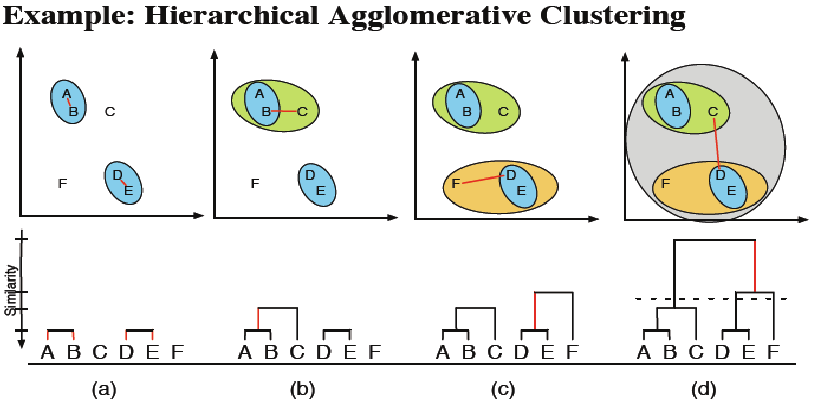
\includegraphics[scale = 0.5]{Figures/hierarchical_clustering.png}
	\caption{Iterative steps for hierarchical agglomerative clustering}
	\label{fig: hac}
\end{figure}
 
\subsection{Challenges}

Unlike other clustering methods, hierarchical clustering does not have any principled way to determine the optimal number of clusters. Thus, we have to determine which of the subtrees are clusters, and which subtrees are only a part of a bigger cluster. If one wishes to turn a dendrogram (lower part of Figure \ref{fig: hac}) into a partition of the space (a clustering), one needs to employ a \textit{stopping criterion}. Common stopping criterions include:
\begin{itemize}
	\item Fixed number of clusters: fix some parameter, $k$, and stop merging clusters as soon as the number of clusters is $k$.
	\item Distance upper bound: fix some $r \in \mathbb{R^+}$. Stop merging as soon as all the between-clusters distances are larger than $r$. We can also set $r$ to be $\alpha \max \{d(x,y): x,y \in \mathbb{X} \}$ for some $\alpha <1$. In that case the stopping criterion is called "scaled distance upper bound."
\end{itemize}

The second stopping criterion basically suggests that we want to stop merging when the cost of merging increases a lot and thus it most likely loses a lot of structure. As such, this leaves us to decide how big a merging cost is acceptable and there is no proven theory to say that this method will often or even usually lead to good choices. In addition, we may also face difficulty in picking the right similarity measure (or linkage) for our data.

%----------------------------------------------------------------------------------------

 
% Chapter 5

\chapter{Empirical Study}
%\setlength{\textfloatsep}{1pt}
%\setlength{\floatsep}{5pt}
%\setlength{\intextsep}{5pt}
\setlength{\belowdisplayskip}{1pt} \setlength{\belowdisplayshortskip}{1pt}
\setlength{\abovedisplayskip}{1pt} \setlength{\abovedisplayshortskip}{1pt}

In this chapter, we will apply the algorithms mentioned previously on the different datasets to study the coordination between nuclear and mitochondrial genomes. Before that, we will describe the data in more detail.

\section{Description of Data}
The data that we have is \textbf{unlabelled} mouse’s gene expression values which are in numeric. The values have also been transformed to $\log_2$, which is a standard practice in computational biology. Since it is unlabelled, and from the plots we cannot identify distinct clusters, we have to apply unsupervised learning (clustering in this case). It is a short time-series, with only 7 time points. Each time point has around $8,000-10,000$ samples. On top of that, these $8,000-10,000$ genes may not exhibit separable or significant clusters so we will look deeper into a special set of genes which are the mitochondrial genes (around $1,100$ samples). We would expect to see more significant separation for this $1,100$ samples. We would also expect that this $1,100$ genes to be highly expressed (higher value) at later time points since they become more abundant in the mitochondrial biogenesis process.

For this report, we will only present results mainly from RNA Crude and RNA Crude Mito as we would expect these pools to be more biologically significant. Furthermore, we will not display all the plots of the different clusters. Instead, we will only present those plots with significantly enriched GO terms. The rest of the results can be found in the appendix \ref{AppendixA}.

\subsection{Exploratory Analysis}
Here we present some basic analysis for our data. From the figures below, we may expect that Gaussian Mixture Model (refer to Section \ref{3.2}) will be useful in clustering our time-series gene expression values since all the plots show that the data follow Gaussian normal distribution. Nonetheless, from these figures, we also see that our hypothesis is not totally true as the mitochondrial genes at later time points are not that highly expressed as compared to the earlier time points. The distribution of the values, the maximum and minimum values are generally similar for all time points. This may pose some problems when we cluster the mitochondrial genes as they may not exhibit distinct properties as we expect.
		
\begin{figure}[H]
\renewcommand{\arraystretch}{0.5}
	\begin{tabular}{ccc}
		\includegraphics[width = 55mm,height=35mm]{Figures/exploratory/hist_RNACru_t0.png} &
		\includegraphics[width = 55mm,height=35mm]{Figures/exploratory/hist_RNACru_t1.png} &
		\includegraphics[width = 55mm,height=35mm]{Figures/exploratory/hist_RNACru_t2.png} \\
		$t_0$ & $t_1$ & $t_2$ \\
		\includegraphics[width = 55mm,height=35mm]{Figures/exploratory/hist_RNACru_t3.png} &
		\includegraphics[width = 55mm,height=35mm]{Figures/exploratory/hist_RNACru_t4.png} &
		\includegraphics[width = 55mm,height=35mm]{Figures/exploratory/hist_RNACru_t5.png} \\ 
		$t_3$ & $t_4$ & $t_5$ \\
		\multicolumn{3}{c}{\includegraphics[width=55mm,height=35mm]{Figures/exploratory/hist_RNACru_t6.png}} \\
	\multicolumn{3}{c}{$t_6$}
	\end{tabular}
\label{fig: HistRNACrude}
\caption{Distribution of $\log_2 RPKM$ values for RNA Crude}
\end{figure}

\begin{figure}[H]
\renewcommand{\arraystretch}{0.5}	
	\begin{tabular}{ccc}
		\includegraphics[width=55mm,height=30mm]{Figures/exploratory/hist_RNACruMito_t0.png} &
		\includegraphics[width=55mm,height=30mm]{Figures/exploratory/hist_RNACruMito_t1.png}&
		\includegraphics[width=55mm,height=30mm]{Figures/exploratory/hist_RNACruMito_t2.png}\\
		$t_0$ & $t_1$ & $t_2$ \\
		\includegraphics[width=55mm,height=30mm]{Figures/exploratory/hist_RNACruMito_t3.png}&
		\includegraphics[width=55mm,height=30mm]{Figures/exploratory/hist_RNACruMito_t4.png}&
		\includegraphics[width=55mm,height=30mm]{Figures/exploratory/hist_RNACruMito_t5.png}\\\
		$t_3$ & $t_4$ & $t_5$ \\
	\multicolumn{3}{c}{\includegraphics[width=55mm,height=30mm]{Figures/exploratory/hist_RNACruMito_t6.png}} \\
\multicolumn{3}{c}{$t_6$}							
	\end{tabular}
\label{fig: HistRNACrudeMito}
\caption{Distribution of $\log_2 RPKM$ values for RNA Crude Mitochondrial Genes}
\end{figure}

\begin{figure}[H]
	\renewcommand{\arraystretch}{0.5}
	\centering
	\begin{tabular}{cc}
		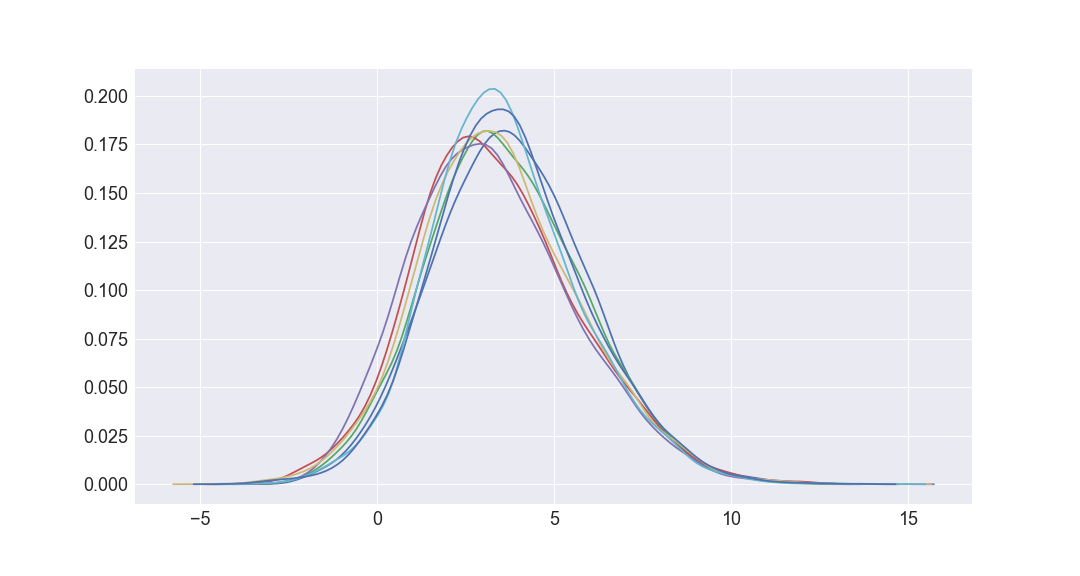
\includegraphics[width=75mm,height=40mm]{Figures/exploratory/kde_RNACru.png}&
		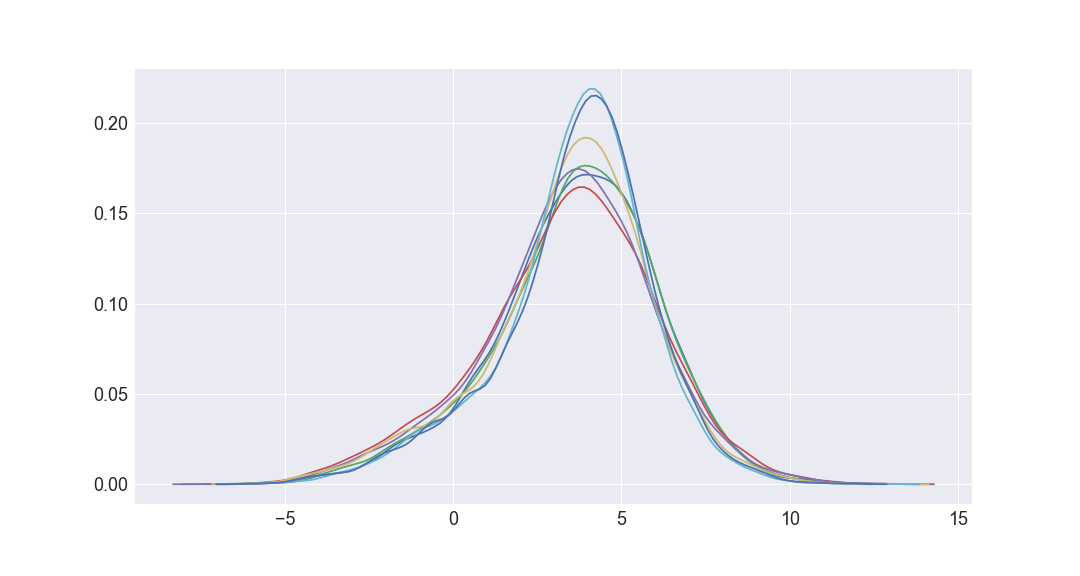
\includegraphics[width=75mm,height=40mm]{Figures/exploratory/kde_RNATot.png} \\
		RNA Crude & RNA Bulk \\
		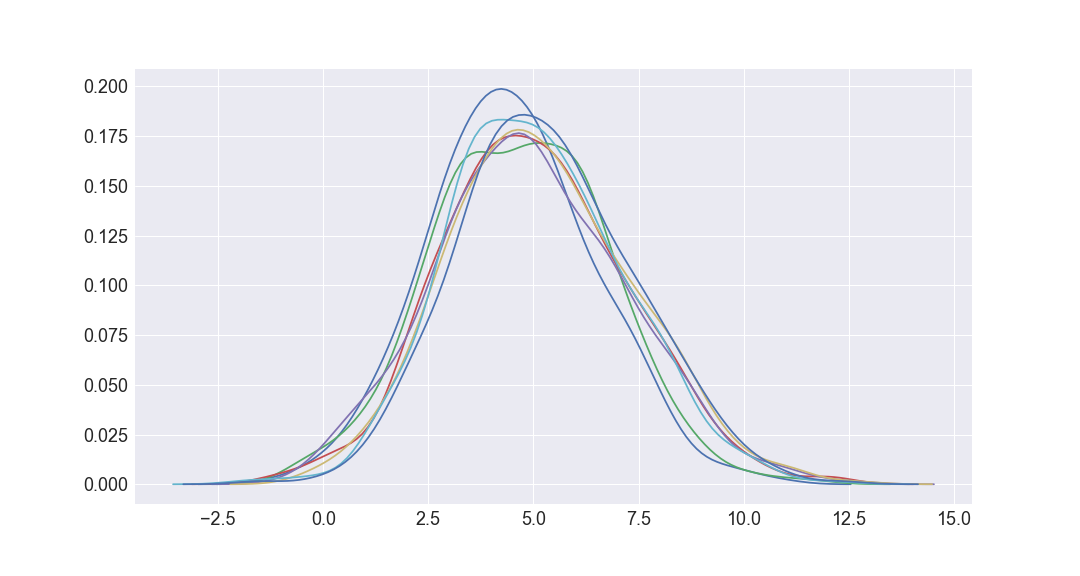
\includegraphics[width=75mm,height=40mm]{Figures/exploratory/kde_RNACruMito.png} &
		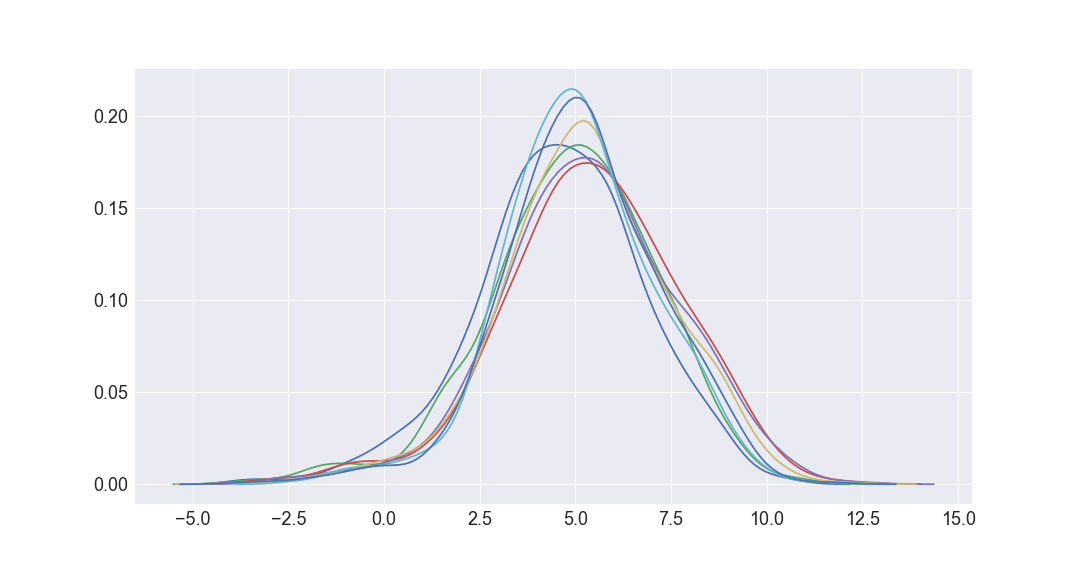
\includegraphics[width=75mm,height=40mm]{Figures/exploratory/kde_RNATotMito.png} \\
		RNA Crude Mitochondria & RNA Bulk Mitochondria
	\end{tabular}
\label{fig: KDE}
\caption{Comparison of the distribution between different datasets}
\end{figure}

\section{STEM}
\subsection{Results}
Here, we use $m=100$ and $c=3$. Using different values for $m$ and $c$ do not give us significant differences for the clustering results. We use $\delta = 0.3$ as the minimum threshold to group similar significant clusters (refer to Section \ref{3.1}). Unfortunately, STEM excludes about $40\%$ of the original pool of genes in its clustering. For RNA Crude, the number of genes considered in the significant clusters are $4894$ genes (before cluster is $8675$ genes). Similarly, for RNA Crude Mito, the number is $420$ genes (before cluster is $911$ genes). Due to this result, we decide that we only take the optimal number of clusters from STEM ($k=19$ for RNA Crude and $k=11$ for RNA Crude Mito) and then use this for the other algorithms. Moreover, we have also transformed the data into log ratios where the ratios are with respect to the expression of the first time point. We still use the original pools ($8675$ and $911$ genes for Crude and Crude Mito, respectively) of genes for the other algorithms.

%----------------------------------------------------------------------------------------

\section{Mixture Model}
\subsection{Results}
%analysis and plots
From the AIC and BIC analysis below (Figure \ref{fig: aic_bic}), we are unable to determine the optimal number of clusters as it seems that the number of clusters keeps increasing whereas from STEM, we find that the number of clusters is actually not that high. Even when we perform this analysis with maximum number of components of $>100$, we are still unable to find the optimum point. For mitochondrial genes which has at most $1000$ data, AIC and BIC analysis still could not help us extract the optimal number of clusters. The reason is probably because of the nature of the data that is not rich enough to develop obvious separable clusters (refer to \ref{2.1}). Another possible reason is that the data simply cannot be modelled as a mixture of Gaussians. As such, we initialize the number of clusters for GMM obtained from STEM and then perform GO analysis for the two covariance matrices. We then perform GO analysis on each of the resulting clusters. Nonetheless, this result may correspond to the inability of STEM to cluster most of the genes (it only clusters $\approx 60 \%$ of the total genes) which means that indeed the data can be divided into many clusters.

\begin{figure}[H]
			\centering	
	\renewcommand{\arraystretch}{0.5}
	\begin{tabular}{cc}

		\includegraphics[width=62mm,height=45mm]{Figures/opt_clust_diff0/thresh_0/RNAcruLogdiff0/RNAcru__aic_diag.png}&
		\includegraphics[width=62mm,height=45mm]{Figures/opt_clust_diff0/thresh_0/RNAcruLogdiff0/RNAcru__bic_diag.png} \\
		AIC Curve(Diagonal) & BIC Curve(Diagonal) \\
			\includegraphics[width=62mm,height=45mm]{Figures/opt_clust_diff0/thresh_0/RNAcruLogdiff0/RNAcru__aic_spherical.png}
				 &
				\includegraphics[width=62mm,height=45mm]{Figures/opt_clust_diff0/thresh_0/RNAcruLogdiff0/RNAcru__bic_spherical.png}	\\
			BIC Curve(Spherical) & BIC Curve(Spherical)  
	\end{tabular}
	\caption{AIC and BIC results for GMM with Diagonal and Spherical covariance matrices for RNA Crude data}
	\label{fig: aic_bic}
\end{figure}

%----------------------------------------------------------------------------------------

\section{K-means}
\subsection{Results}
%analysis&plots
Similar to GMM, we are unable to determine the optimum number of clusters for k-means algorithm from both the elbow curve and gap statistics analysis (Figure \ref{fig:elbowGap}). \textit{K-means} may face the same problem like GMM that the data may not be rich enough to develop separable clusters for \textit{k-means}. Another possible reasons is that euclidean distance may not be a good measure. As such, we will proceed with using optimal number of clusters obtained from STEM and the perform \textit{k-means} algorithm to the data with this initial number of clusters. Then, we perform GO analysis on the resulting clusters.

\begin{figure}[H]
	\centering
	\renewcommand{\arraystretch}{0.5}
	\begin{tabular}{cc}
		\includegraphics[width=75mm,height=45mm]{Figures/opt_clust_diff0/thresh_0/RNAcruLogdiff0/RNACru_elbow.png} &
		\includegraphics[width=75mm,height=45mm]{Figures/opt_clust_diff0/thresh_0/RNAcruLogdiff0/RNACru_gap.png} \\
		Elbow Curve(RNA Crude) & Gap Statistic Curve(RNA Crude) \\
		\includegraphics[width=75mm,height=45mm]{Figures/opt_clust_diff0/thresh_0/RNAcruMitoLogdiff0/RNACruMito_elbow.png} &				\includegraphics[width=75mm,height=45mm]{Figures/opt_clust_diff0/thresh_0/RNAcruMitoLogdiff0/RNACruMito_gap.png} \\
		Elbow Curve(RNA Crude Mito) & Gap Statistic Curve(RNA Crude Mito)
	\end{tabular}
\caption{Finding Optimal $k$ for \textit{k-means}}
\label{fig:elbowGap}
\end{figure}

%----------------------------------------------------------------------------------------

\section{Hierarchical Clustering}
\subsection{Results}
As mentioned in the previous chapter (Section \ref{4.4}), we will not be able to determine the optimal number of clusters from the dendrograms. Similar to the other algorithms, we will use $k$ obtained from STEM. In this report, we will only show the plots for HAC with Complete linkage as it gives the best results (found in Appendix \ref{AppendixA}).

%----------------------------------------------------------------------------------------
\section{Comparison of Algorithms} \label{5.2}
In this section, we use $k=19$ and $k=11$ for RNA Crude and RNA Crude Mito respectively when we apply the other clustering algorithms. From the results below (Table \ref{tab: number of genes RNA Crude} and Table \ref{tab: number of genes RNA Crude Mito}), we can see that the number of genes that fall into each cluster for different algorithms is actually quite similar (except for HAC (Comp)), especially when the total number of genes in the whole dataset is small (for RNA Crude Mito).
\begin{table}[H]
	\centering
	\begin{tabular}{lcccc}
		\hline
		\textbf{Cluster} & \textbf{K-means} & \textbf{GMM (Sph)} & \textbf{GMM (Comp)} & \textbf{HAC (Comp)} \\ \hline
		\textbf{1}       & 791              & 947                & 851                 & 2123                \\ \hline
		\textbf{2}       & 756              & 925                & 814                 & 978               \\ \hline
		\textbf{3}       & 751              & 897                & 805                 & 872                 \\ \hline
		\textbf{4}       & 678              & 720                & 712                 & 832                 \\ \hline
		\textbf{5}       & 666              & 619                & 667                 & 756                 \\ \hline
		\textbf{6}       & 658              & 554                & 636                 & 475                 \\ \hline
		\textbf{7}       & 625              & 544                & 523                 & 456                 \\ \hline
		\textbf{8}       & 573              & 480                & 503                 & 430                 \\ \hline
		\textbf{9}       & 532              & 457                & 489                 & 362                 \\ \hline
		\textbf{10}      & 492              & 455                & 473                 & 357                 \\ \hline
		\textbf{11}      & 469              & 410                & 408                 & 188                 \\ \hline
		\textbf{12}      & 460              & 355                & 376                 & 181                 \\ \hline
		\textbf{13}      & 324              & 346                & 371                 & 173                 \\ \hline
		\textbf{14}      & 276              & 243                & 334                 & 110                 \\ \hline
		\textbf{15}      & 227              & 225                & 300                 & 104                 \\ \hline
		\textbf{16}      & 178              & 212                & 175                 & 97                  \\ \hline
		\textbf{17}      & 96               & 122                & 96                  & 89                  \\ \hline
		\textbf{18}      & 69               & 100                & 82                  & 47                  \\ \hline
		\textbf{19}      & 35               & 45                 & 41                  & 45                  \\ \hline
	\end{tabular}
	\caption{Gene count in each cluster for the different algorithms \\
	($k=19$), total number of genes = $8675$}
	\label{tab: number of genes RNA Crude}
\end{table}

\begin{table}[H]
	\centering
	\begin{tabular}{lcccc}
		\hline
		\textbf{Cluster} & \textbf{K-means} & \textbf{GMM (Sph)} & \textbf{GMM (Diag)} & \textbf{HAC (Comp)}  \\ \hline
		\textbf{1}       & 134              & 140                & 121                 & 357                \\ \hline
		\textbf{2}       & 126              & 122                & 110                 & 98                 \\ \hline
		\textbf{3}       & 111              & 102                & 107                 & 84                 \\ \hline
		\textbf{4}       & 99               & 102                & 100                  & 76                   \\ \hline
		\textbf{5}       & 82               & 99                 & 100                  & 76                  \\ \hline
		\textbf{6}       & 82               & 78                 & 89                  & 69                   \\ \hline
		\textbf{7}       & 77               & 77                 & 88                  & 41                   \\ \hline
		\textbf{8}       & 69               & 57                 & 87                  & 40                  \\ \hline
		\textbf{9}       & 55               & 56                 & 56                  & 32                  \\ \hline
		\textbf{10}      & 54               & 48                 & 35                  & 28                  \\ \hline
		\textbf{11}      & 20              & 30                 & 18                  & 10                   \\ \hline
	\end{tabular}
	\caption{Gene count in each cluster for the different algorithms \\
	($k=11$), total number of genes = $911$}
	\label{tab: number of genes RNA Crude Mito}
\end{table}

\subsection{GO Analysis}
In this section, we will only show the results for RNA Crude Mito. For each of the $11$ clusters we get from the various algorithms, we perform GO analysis (we focus on \textit{biological process} (bp), \textit{cellular compartment} (cc) and \textit{KEGG pathway} (KEGG)). We use \textit{clusterprofiler} \cite{clusterprofiler} to perform our GO analysis. Our GO analysis shows that majority of the clusters indeed contain genes that share similar biological properties. This proves the earlier proposition that genes with similar biological properties may be found in the same cluster in terms of their expression values. Then, we mostly only include GO terms that are related to mitochondrial biogenesis. Furthermore, this confirms our earlier belief that traditional clustering algorithms such as GMM, K-means and HAC can still be useful in clustering time-series data, even when it is short.

When we perform GO analysis on clusters from STEM algorithm($\approx$ 50\% data) we do not get as many enriched clusters as we get from the other algorithms. This may show that STEM removes important genes that should have been clustered into one of the significant clusters. Interestingly, some enriched GO terms appear in multiple clusters, such as \textbf{mitochondrial inner membrane, OXPHOS, mitochondrial gene expression}. This means that there may be interaction between clusters. Yet, it may also be expected that these are common mitochondrially-related GO terms. By analyzing these enriched GO terms with the genes involved in each GO term further such as by incorporating additional biological data, we may then be able to make better conclusion on our objective. 

Here is a brief summary of the GO analysis for RNA Crude Mito:
\begin{itemize}
	\item K-means
	\begin{itemize}
		\item Cluster 3 (110 genes): cc (mitochondrial inner membrane, organelle inner membrane), KEGG (carbon metabolism, TCA cycle, OXPHOS)
		\item Cluster 5 (81 genes): bp (mitochondrial transport, mitochondrial gene expression), cc (mitochondrial inner membrane, mitochondrial matrix), KEGG (ribosome, OXPHOS, Parkinson's disease)		
		\item Cluster 7 (76 genes): bp (cellular respiration, mitochondrial respiratory chain complex I assembly), cc (mitochondrial inner membrane, organelle inner membrane), KEGG (OXPHOS, Parkinson's disease, Alzheimer's disease)
		\item Cluster 11 (19 genes): cc (inner mitochondrial membrane protein complex, Mitochondrial protein complext), KEGG (OXPHOS, Parkinson's disease, Thermogenesis)
	\end{itemize}
	\item GMM (Diagonal)
	\begin{itemize}
		\item Cluster 4 (99 genes): cc (mitochondrial inner membrane, organelle inner membrane, mitochondrial membrane), KEGG (OXPHOS, carbon metabolism, Huntington's diseases)
		\item Cluster 5 (99 genes): bp (mitochondrial transport, mitochondrial gene expression), cc (mitochondrial matrix, mitochondrial inner membrane, organnelle inner membrane), KEGG (OXPHOS, Thermogenesis)
		\item Cluster 6 (88 genes)8: cc (mitochondrial inner membrane, organelle inner membrane, mitochodrial protein complex), KEGG (OXPHOS, Parkinson's disease, Alzheimers' disease)
		\item Cluster 8 (86 genes): bp (mitochondrial transport, mitochondrial gene expression), cc (mitochondrial matrix, mitochondrial inner membrane)
		\item Cluster 10 (34 genes): cc (inner mitochondrial membrane, mitochondrial protein complex), KEGG (OXPHOS, Parkinson's disease, Alzheimers' disease)
	\end{itemize}
	\item GMM (Spherical)
	\begin{itemize}
		\item Cluster 3 (101 genes): cc (mitochondrial inner membrane, organelle inner membrane), KEGG (OXPHOS, carbon metabolism, Huntington's disease, Parkinson's disease)		
		\item Cluster 5 (98 genes): bp (mitochondrial transport, mitochondrial gene expression), cc (mitochondrial matrix, organelle ribosome, mitochondrial inner membrane), KEGG (ribosome, Huntington's disease)
		\item Cluster 7 (76 genes): cc (mitochondrial inner membrane, mitochondrial protein complex), KEGG (OXPHOS, Parkinson's disease, Alzheimer's disease) 
		\item Cluster 10 (47 genes): cc (mitochondrial protein complex, organelle inner membrane), KEGG (OXPHOS, Parkinson's disease, Alzheimer's disease)		
	\end{itemize}
	\item HAC (Complete)
	\begin{itemize}
		\item Cluster 1 (357 genes):  cc (mitochondrial inner membrane, organelle inner membrane), KEGG (OXPHOS, thermogenesis, carbon metabolism)
		\item Cluster 2 (98 genes): bp (purine ribonucleoside triphosphate metabolic process, ribonucleoside triphosphate metabolic process), cc (organelle inner membrane, mitochondrial inner membrane, mitochondrial matrix), KEGG (Parkinson's disease, OXPHOS)
		\item Cluster 3 (84 genes): bp (mitochondrial RNA metabolic process, mitochondrial respiratory chain complex assembly), cc (mitochondrial matrix, mitochondrial inner membrane)
		\item Cluster 4 (76 genes): bp (mitochondrial respiratory chain complex assembly, cellular respiratory), cc (mitochondrial inner membrane, organelle inner membrane), KEGG (OXPHOS, thermogenesis)
	\end{itemize}
		
\end{itemize}

Similar enriched GO terms and other terms also appear when we perform GO analysis for RNA Crude (results are exluded). The cluster plots for the above summary can be found below:

\begin{figure}[H]
	\label{fig: cluster GO plots}
	\renewcommand{\arraystretch}{0.5}
	\begin{tabular}{cccc}
		\includegraphics[width=35mm,height=30mm]{Figures/rna_cru_mito_clust_2/KMeans_cluster_8_111.png} &
		\includegraphics[width=35mm,height=30mm]{Figures/rna_cru_mito_clust_2/KMeans_cluster_4_82.png} &		
		\includegraphics[width=35mm,height=30mm]{Figures/rna_cru_mito_clust_2/KMeans_cluster_7_77.png} &		
		\includegraphics[width=35mm,height=30mm]{Figures/rna_cru_mito_clust_2/KMeans_cluster_5_20.png} \\		
		110 genes & 81 genes & 76 genes & 19 genes \\
		\includegraphics[width=35mm,height=30mm]{Figures/rna_cru_mito_clust_2/GMM-diag_cluster_5_100.png} &
		\includegraphics[width=35mm,height=30mm]{Figures/rna_cru_mito_clust_2/GMM-diag_cluster_9_100.png} &
		\includegraphics[width=35mm,height=30mm]{Figures/rna_cru_mito_clust_2/GMM-diag_cluster_8_89.png} &
		\includegraphics[width=35mm,height=30mm]{Figures/rna_cru_mito_clust_2/GMM-diag_cluster_6_35.png} \\
		99 genes & 99 genes & 88 genes & 34 genes \\
		\includegraphics[width=35mm,height=30mm]{Figures/rna_cru_mito_clust_2/GMM-sph_cluster_1_102.png} &
		\includegraphics[width=35mm,height=30mm]{Figures/rna_cru_mito_clust_2/GMM-sph_cluster_3_99.png} &		
		\includegraphics[width=35mm,height=30mm]{Figures/rna_cru_mito_clust_2/GMM-sph_cluster_6_77.png} &		
		\includegraphics[width=35mm,height=30mm]{Figures/rna_cru_mito_clust_2/GMM-sph_cluster_2_48.png} \\
		101 genes & 98 genes & 76 genes & 47 genes \\
		\includegraphics[width=35mm,height=30mm]{Figures/rna_cru_mito_clust/HAC-comp_Cluster_2_357.png} &
		\includegraphics[width=35mm,height=30mm]{Figures/rna_cru_mito_clust/HAC-comp_Cluster_3_98.png} &
		\includegraphics[width=35mm,height=30mm]{Figures/rna_cru_mito_clust/HAC-comp_Cluster_1_84.png} &
		\includegraphics[width=35mm,height=30mm]{Figures/rna_cru_mito_clust/HAC-comp_Cluster_5_76.png} \\
		357 genes & 98 genes & 84 genes & 76 genes						
	\end{tabular}
\caption{Plots comparison for the $4$ enriched clusters\\
			In order of appearance: K-means, GMM (Diagonal), GMM (Spherical), HAC (Ward)}
\end{figure}

%----------------------------------------------------------------------------------------

\section{Performance Evaluation}
In this section, we compare the performances of the different clustering algorithm with the assumption that STEM gives the optimal clustering. Here, we cannot use the whole pool of genes as STEM does not consider about half of these genes to be significant. Thus, we pick the genes that are considered significant by STEM and then apply the other clustering algorithms to these sets of genes. Then, we compare the performances of each clustering algorithm with using the two metrics described earlier (\textit{clustering accuracy} and \textit{ME distance}, refer to Section \ref{2.3}).  
\begin{table}[H]
	\centering
		\begin{tabular}{lcccccccc}
			\hline
			& \multicolumn{2}{c}{\textbf{RNA Bulk}} & \multicolumn{2}{c}{\textbf{RNA Bulk (Mito)}} & \multicolumn{2}{c}{\textbf{RNA Crude}} & \multicolumn{2}{c}{\textbf{RNA Crude (Mito)}} \\ \hline
			\textbf{Algorithm}  & \textbf{CA}       & \textbf{ME}       & \textbf{CA}           & \textbf{ME}          & \textbf{CA}        & \textbf{ME}       & \textbf{CA}           & \textbf{ME}           \\ \hline
			\textbf{K-means}    & 56.37             & 68.17             & 66.77                 & 59.91                & 48.39    & 72.60             & 45.95                 & 68.81                 \\  \hline
			\textbf{GMM (Full)} & 50.87             & 71.41             & 59.15                 & 58.84       & 51.70              & 71.00             & 53.81                 & 64.76        \\
			\textbf{GMM (Diag)} & 52.79             & 72.31             & 68.90                 & 59.15                & 44.34              & 76.24    & 42.86                 & 71.67               \\
			\textbf{GMM (Sph)}  & 57.23            & 70.55             & 66.92                 & 60.52                & 53.11              & 72.00             & 48.10                 & 67.86                 \\ \hline
			\textbf{HAC (Ward)} & 53.17             & 70.75    & 63.41                 &60.52               & 47.10              & 73.03             & 43.10                 & 71.43                 \\
			\textbf{HAC (Comp)} & \underline{71.68}    & 49.61             & \underline{78.51}        & \underline{31.55}               & \underline{67.94}              & 49.94             & \underline{71.43}       & \underline{44.76}                 \\
			\textbf{HAC (Ave)}  & 66.40             & \underline{38.88}            & 73.48                 & 33.84                & 64.73              & \underline{44.79}             & 61.43                 & \underline{44.76}                
	\end{tabular}
	\caption{Performance evaluation for the different algorithms (in \%), the underlined values are the best performing algorithm for that particular class of clustering}
	\label{tab: performance}
\end{table}

From the Table \ref{tab: performance} above, we can see that there is no algorithm that outperforms the rest for all the datasets. As expected, HAC with Complete and Average as the linkage outperforms the other algorithms since they use correlation coefficient as the distance metric just like STEM. Another interesting result is that some of the algorithms perform worse for RNA Crude (Mito) when the size of the data is smaller. 
% Chapter 6

\chapter{Conclusion}
\setlength{\belowdisplayskip}{1pt} \setlength{\belowdisplayshortskip}{1pt}
\setlength{\abovedisplayskip}{1pt} \setlength{\abovedisplayshortskip}{1pt}
\section{Summary}
\subsection{STEM To Determine Number of Clusters}
We pick STEM as the algorithm that provides the optimum clustering due to a few reasons:
\begin{itemize}
	\item Only STEM that can give us optimal number of clusters from the statistical test
	\item STEM takes into account the sequential nature of time-series data
	\item STEM generates profiles that are independent of the data
	\item Profiles generated by STEM tells us the dynamic between successive time points
\end{itemize}
Nonetheless, since STEM also computes the statistical significance of each cluster, it can exclude many genes which could have been clustered. This omits the possibility of having biologically significant clusters yet not statistically significant clusters as shown in the GO analysis for the other algorithms. Hence, our proposal is that to perform STEM and then extract the optimal number of clusters ($k$) from it. Thereafter, we use $k$ as the initial input for other clustering algorithms and perform GO analysis on the resulting clusters. On the other hand, if the removal of many genes corresponds to removal of noise, STEM may then be used to filter out noise.

\subsection{No Algorithm Performs Better For All Data}
Our results show that no algorithm performs better for all situations. From all the clusters generated by each algorithm, there are always a mix between biologically and statistically meaningful clusters and those that are not. It is also difficult to conclude on what kind of situation or data where one algorithm can perform better than rest. We may need to further preprocess the data to see whether it can improve the performance of each algorithm. As expected, Hierarchical Clustering with Complete and Average linkage performs better than the other algorithms.

\section{Further Work}
\subsection{Different Algorithms}
There are still plenty of clustering algorithms out there that can be used to cluster short time-series data. One possible future plan is to improve the algorithms that we have used previously, such as by incorporating additional data or prior; adjusting the parameters. Here we mention briefly some algorithms that have been improved or modified to cluster short time-series gene expression data:
\subsubsection{Explore On Soft Clustering}
All the algorithms above are considered hard clustering, which means one gene cannot belong to more than one cluster. In reality, one gene can belong to multiple biological groups and thus, may belong to more than one cluster. For this aspect, we can perform Fuzzy-clustering algorithm, a popular soft clustering algorithm. Fuzzy-clustering, modified for short time-series \cite{Moller-Levet2003} has also been used to study the dynamic of gene expression values with short time points. 
\subsubsection{Bayesian Approach}
We can also consider to study variational Bayesian estimation of Gaussian Mixture model \cite{Jia2008} that may improve the performance of GMM. We implement the technique of variational inference, which is an extension of expectation-maximization that maximizes a lower bound on model evidence (including priors) instead of data likelihood. Due to its Bayesian nature, this model allows us to specify a concentration parameter: weight concentration prior, which helps affect the number of components in the model. Furthermore, high concentration parameter not only leads to more active components in the mixture, but also more uniform weights, which may be useful.
\subsection{Interaction Between Clusters}
As mentioned in Section \ref{5.2}, there may be interaction between clusters which will give more insights on our clustering. One method that has been used is an improvement of HAC, \textit{Fast Optimal Leaf Ordering For Hierarchical Clustering} \cite{fasthac}. Optimal leaf ordering causes input elements that are highly correlated in a cluster to appear in the middle of the linear ordering of the cluster, while marginally related elements are on the borders of the cluster. This improvement reorders the leaves in HAC which gives a more understandable visualizations and hence, helps reveal more biological structures. These relationships are very important in time series data analysis. 
\subsection{Other Distance Measures}
There are also plenty of distance or similarity measures that can be used when we want to cluster time-series data such dynamic time warping distance, short time-series distance developed for Fuzzy-clustering \cite{Moller-Levet2003} and many other. 


%----------------------------------------------------------------------------------------
%	THESIS CONTENT - APPENDICES
----------------------------------------------------------------------------------------

\appendix % Cue to tell LaTeX that the following "chapters" are Appendices

% Include the appendices of the thesis as separate files from the Appendices folder
% Uncomment the lines as you write the Appendices

% Appendix A

\chapter{Plots For RNA Bulk Mito} % Main appendix title

\label{AppendixA} % For referencing this appendix elsewhere, use \ref{AppendixA}

\begin{figure}[H]
	\renewcommand{\arraystretch}{0.5}
	\begin{tabular}{ccc}
		\includegraphics[width=55mm,height=35mm]{Figures/rna_tot_mito_clust/STEM_Cluster_0_157.png} & \includegraphics[width=55mm,height=35mm]{Figures/rna_tot_mito_clust/STEM_Cluster_1_155.png} & \includegraphics[width=55mm,height=35mm]{Figures/rna_tot_mito_clust/STEM_Cluster_2_71.png} \\
		(1) 157 genes & (2) 155 genes & (3) 71 genes \\
		\includegraphics[width=55mm,height=35mm]{Figures/rna_tot_mito_clust/STEM_Cluster_3_44.png} & \includegraphics[width=55mm,height=35mm]{Figures/rna_tot_mito_clust/STEM_Cluster_4_61.png} &
		\includegraphics[width=55mm,height=35mm]{Figures/rna_tot_mito_clust/STEM_Cluster_5_57.png} \\
		(4) 44 genes & (5) 61 genes & (6) 57 genes \\
		\includegraphics[width=55mm,height=35mm]{Figures/rna_tot_mito_clust/STEM_Cluster_6_42.png} &
		\includegraphics[width=55mm,height=35mm]{Figures/rna_tot_mito_clust/STEM_Cluster_7_30.png} & 
		\includegraphics[width=55mm,height=35mm]{Figures/rna_tot_mito_clust/STEM_Cluster_8_20.png}\\ 
		(7) 42 genes & (8) 30 genes & (9) 20 genes \\
		\multicolumn{3}{c}{\includegraphics[width=55mm,height=35mm]{Figures/rna_tot_mito_clust/STEM_Cluster_9_19.png}} \\
		\multicolumn{3}{c}{(10) 19 genes}
	\end{tabular}
	\caption{Clustering Results for STEM}
\end{figure}


\begin{figure}[H]
	\renewcommand{\arraystretch}{0.5}
	\begin{tabular}{ccc}
		\includegraphics[width=55mm,height=35mm]{Figures/rna_tot_mito_clust/KMeans_Cluster_4_196.png} &
		\includegraphics[width=55mm,height=35mm]{Figures/rna_tot_mito_clust/KMeans_Cluster_5_177.png} &
		\includegraphics[width=55mm,height=35mm]{Figures/rna_tot_mito_clust/KMeans_Cluster_3_145.png}	\\
		(1) 196 genes & (2) 177 genes & (3) 145 genes \\
		\includegraphics[width=55mm,height=35mm]{Figures/rna_tot_mito_clust/KMeans_Cluster_1_132.png} &
		\includegraphics[width=55mm,height=35mm]{Figures/rna_tot_mito_clust/KMeans_Cluster_2_124.png} &
		\includegraphics[width=55mm,height=35mm]{Figures/rna_tot_mito_clust/KMeans_Cluster_9_108.png}		\\
		(4) 132 genes & (5) 124 genes & (6) 108 genes \\
		\includegraphics[width=55mm,height=35mm]{Figures/rna_tot_mito_clust/KMeans_Cluster_8_54.png} &
		\includegraphics[width=55mm,height=35mm]{Figures/rna_tot_mito_clust/KMeans_Cluster_6_46.png} &
		\includegraphics[width=55mm,height=35mm]{Figures/rna_tot_mito_clust/KMeans_Cluster_0_15.png} \\
		(7) 54 genes & (8) 46 genes & (9) 15 genes \\
		\multicolumn{3}{c}{\includegraphics[width=55mm,height=35mm]{Figures/rna_tot_mito_clust/KMeans_Cluster_7_9.png}} \\
		\multicolumn{3}{c}{(10) 9 genes}			
	\end{tabular}
	\caption{Clustering results for k-means}
\end{figure}

\begin{figure}[H]
	\renewcommand{\arraystretch}{0.5}
	\begin{tabular}{ccc}
		\includegraphics[width=55mm,height=35mm]{Figures/rna_tot_mito_clust/GMM-diag_Cluster_4_192.png} &
		\includegraphics[width=55mm,height=35mm]{Figures/rna_tot_mito_clust/GMM-diag_Cluster_0_187.png} &
		\includegraphics[width=55mm,height=35mm]{Figures/rna_tot_mito_clust/GMM-diag_Cluster_5_172.png}  \\
		(1) 192 genes & (2) 187 genes & (3) 172 genes \\
		\includegraphics[width=55mm,height=35mm]{Figures/rna_tot_mito_clust/GMM-diag_Cluster_7_137.png}  &
		\includegraphics[width=55mm,height=35mm]{Figures/rna_tot_mito_clust/GMM-diag_Cluster_1_124.png} &
		\includegraphics[width=55mm,height=35mm]{Figures/rna_tot_mito_clust/GMM-diag_Cluster_6_61.png} \\
		(4) 137 genes & (5) 124 genes & (6) 61 genes \\
		\includegraphics[width=55mm,height=35mm]{Figures/rna_tot_mito_clust/GMM-diag_Cluster_2_53.png} &
		\includegraphics[width=55mm,height=35mm]{Figures/rna_tot_mito_clust/GMM-diag_Cluster_9_51.png} &
		\includegraphics[width=55mm,height=35mm]{Figures/rna_tot_mito_clust/GMM-diag_Cluster_8_19.png} \\
		(7) 53 genes & (8) 51 genes & (9) 19 genes \\
		\multicolumn{3}{c}{\includegraphics[width=55mm,height=35mm]{Figures/rna_tot_mito_clust/GMM-diag_Cluster_3_10.png}} \\
		\multicolumn{3}{c}{(10) 10 genes}		
	\end{tabular}
	\caption{Clustering results for GMM(Diagonal)}
\end{figure}


\begin{figure}[H]
	\renewcommand{\arraystretch}{0.5}
	\begin{tabular}{ccc}
		\includegraphics[width=55mm,height=35mm]{Figures/rna_tot_mito_clust/GMM-sph_Cluster_6_205.png} &
		\includegraphics[width=55mm,height=35mm]{Figures/rna_tot_mito_clust/GMM-sph_Cluster_7_172.png} &
		\includegraphics[width=55mm,height=35mm]{Figures/rna_tot_mito_clust/GMM-sph_Cluster_9_144.png} \\
		(1) 205 genes & (2) 172 genes & (3) 144 genes \\				\includegraphics[width=55mm,height=35mm]{Figures/rna_tot_mito_clust/GMM-sph_Cluster_3_121.png} &
		\includegraphics[width=55mm,height=35mm]{Figures/rna_tot_mito_clust/GMM-sph_Cluster_2_120.png} &
		\includegraphics[width=55mm,height=35mm]{Figures/rna_tot_mito_clust/GMM-sph_Cluster_4_88.png}	\\
		(4) 121 genes & (5) 120 genes & (6) 88 genes \\
		\includegraphics[width=55mm,height=35mm]{Figures/rna_tot_mito_clust/GMM-sph_Cluster_0_83.png} &
		\includegraphics[width=55mm,height=35mm]{Figures/rna_tot_mito_clust/GMM-sph_Cluster_8_43.png} &
		\includegraphics[width=55mm,height=35mm]{Figures/rna_tot_mito_clust/GMM-sph_Cluster_1_20.png}	\\
		(7) 83 genes & (8) 43 genes & (9) 20 genes \\
		\multicolumn{3}{c}{\includegraphics[width=55mm,height=35mm]{Figures/rna_tot_mito_clust/GMM-sph_Cluster_5_10.png}} \\
		\multicolumn{3}{c}{(10) 10 genes}							 			
	\end{tabular}
	\caption{Clustering results for GMM(Spherical)}
\end{figure}

\begin{figure}[H]
	\renewcommand{\arraystretch}{0.5}
	\begin{tabular}{ccc}
		\includegraphics[width=55mm,height=35mm]{Figures/rna_tot_mito_clust/HAC-comp_Cluster_4_361.png} &
		\includegraphics[width=55mm,height=35mm]{Figures/rna_tot_mito_clust/HAC-comp_Cluster_2_175.png} &
		\includegraphics[width=55mm,height=35mm]{Figures/rna_tot_mito_clust/HAC-comp_Cluster_3_132.png} \\
		(1) 361 genes & (2) 175 genes & (3) 132 genes \\ 
		\includegraphics[width=55mm,height=35mm]{Figures/rna_tot_mito_clust/HAC-comp_Cluster_8_87.png} &
		\includegraphics[width=55mm,height=35mm]{Figures/rna_tot_mito_clust/HAC-comp_Cluster_1_81.png} &
		\includegraphics[width=55mm,height=35mm]{Figures/rna_tot_mito_clust/HAC-comp_Cluster_9_73.png} \\
		(4) 87 genes & (5) 81 genes & (6) 73 genes \\
		\includegraphics[width=55mm,height=35mm]{Figures/rna_tot_mito_clust/HAC-comp_Cluster_0_47.png} &
		\includegraphics[width=55mm,height=35mm]{Figures/rna_tot_mito_clust/HAC-comp_Cluster_7_27.png} &
		\includegraphics[width=55mm,height=35mm]{Figures/rna_tot_mito_clust/HAC-comp_Cluster_6_14.png} \\
		(7) 47 genes & (8) 27 genes & (9) 14 genes \\
\multicolumn{3}{c}{\includegraphics[width=55mm,height=35mm]{Figures/rna_tot_mito_clust/HAC-comp_Cluster_5_9.png}} \\
\multicolumn{3}{c}{(10) 9 genes}
	\end{tabular}
	\caption{Clustering results for HAC (Complete)}
\end{figure}

\chapter{Plots For RNA Crude Mito}
\begin{figure}[H]
	\renewcommand{\arraystretch}{0.5}
	\begin{tabular}{ccc}
		\includegraphics[width=55mm,height=35mm]{Figures/rna_cru_mito_clust/STEM_Cluster_0_138.png} &
		\includegraphics[width=55mm,height=35mm]{Figures/rna_cru_mito_clust/STEM_Cluster_1_18.png} &
		\includegraphics[width=55mm,height=35mm]{Figures/rna_cru_mito_clust/STEM_Cluster_2_48.png} \\
		(1) 137 genes & (2) 17 genes & (3) 47 genes \\
		\includegraphics[width=55mm,height=35mm]{Figures/rna_cru_mito_clust/STEM_Cluster_3_44.png} & 						
		\includegraphics[width=55mm,height=35mm]{Figures/rna_cru_mito_clust/STEM_Cluster_4_43.png} &
		\includegraphics[width=55mm,height=35mm]{Figures/rna_cru_mito_clust/STEM_Cluster_5_35.png} \\
		(4) 43 genes & (5) 42 genes & (6) 34 genes \\
		\includegraphics[width=55mm,height=35mm]{Figures/rna_cru_mito_clust/STEM_Cluster_6_22.png} &
		\includegraphics[width=55mm,height=35mm]{Figures/rna_cru_mito_clust/STEM_Cluster_7_21.png} &
		\includegraphics[width=55mm,height=35mm]{Figures/rna_cru_mito_clust/STEM_Cluster_8_19.png} \\
		(7) 21 genes & (8) 20 genes & (9) 8 genes \\
		\includegraphics[width=55mm,height=35mm]{Figures/rna_cru_mito_clust/STEM_Cluster_9_18.png} &
		\includegraphics[width=55mm,height=35mm]{Figures/rna_cru_mito_clust/STEM_Cluster_10_14.png} &
		\\
		(10) 17 genes & (11) 13 genes &
	\end{tabular}
	\caption{Clustering results for STEM}
\end{figure}

\begin{figure}[H]
	\renewcommand{\arraystretch}{0.5}
	\begin{tabular}{ccc}
		\includegraphics[width=55mm,height=35mm]{Figures/rna_cru_mito_clust_2/KMeans_cluster_0_82.png} &
		\includegraphics[width=55mm,height=35mm]{Figures/rna_cru_mito_clust_2/KMeans_cluster_1_99.png} &
		\includegraphics[width=55mm,height=35mm]{Figures/rna_cru_mito_clust_2/KMeans_cluster_2_134.png} \\
		(1) 81 genes & (2) 98 genes & (3) 133 genes \\
		\includegraphics[width=55mm,height=35mm]{Figures/rna_cru_mito_clust_2/KMeans_cluster_3_54.png} &
		\includegraphics[width=55mm,height=35mm]{Figures/rna_cru_mito_clust_2/KMeans_cluster_4_82.png} &
		\includegraphics[width=55mm,height=35mm]{Figures/rna_cru_mito_clust_2/KMeans_cluster_5_20.png} \\
		(4) 53 genes & (5) 81 genes & (6) 19 genes \\
		\includegraphics[width=55mm,height=35mm]{Figures/rna_cru_mito_clust_2/KMeans_cluster_6_57.png} &
		\includegraphics[width=55mm,height=35mm]{Figures/rna_cru_mito_clust_2/KMeans_cluster_7_77.png} &
		\includegraphics[width=55mm,height=35mm]{Figures/rna_cru_mito_clust_2/KMeans_cluster_8_111.png} \\
		(7) 56 genes & (8) 76 genes & (9) 110 genes \\
		\includegraphics[width=55mm,height=35mm]{Figures/rna_cru_mito_clust_2/KMeans_cluster_9_69.png} &
		\includegraphics[width=55mm,height=35mm]{Figures/rna_cru_mito_clust_2/KMeans_cluster_10_126.png} &
		\\
		(10) 68 genes & (11) 125 genes &
	\end{tabular}
	\caption{Clustering results for K-means}
\end{figure}

\begin{figure}[H]
	\renewcommand{\arraystretch}{0.5}
	\begin{tabular}{ccc}
		\includegraphics[width=55mm,height=35mm]{Figures/rna_cru_mito_clust_2/GMM-diag_cluster_0_87.png} &
		\includegraphics[width=55mm,height=35mm]{Figures/rna_cru_mito_clust_2/GMM-diag_cluster_1_107.png} &
		\includegraphics[width=55mm,height=35mm]{Figures/rna_cru_mito_clust_2/GMM-diag_cluster_2_110.png} \\
		(1) 86 genes & (2) 106 genes & (3) 109 genes \\
		\includegraphics[width=55mm,height=35mm]{Figures/rna_cru_mito_clust_2/GMM-diag_cluster_3_121.png} &
		\includegraphics[width=55mm,height=35mm]{Figures/rna_cru_mito_clust_2/GMM-diag_cluster_4_18.png} &
		\includegraphics[width=55mm,height=35mm]{Figures/rna_cru_mito_clust_2/GMM-diag_cluster_5_100.png} \\
		(4) 120 genes & (5) 17 genes & (6) 99 genes \\
		\includegraphics[width=55mm,height=35mm]{Figures/rna_cru_mito_clust_2/GMM-diag_cluster_6_35.png} &
		\includegraphics[width=55mm,height=35mm]{Figures/rna_cru_mito_clust_2/GMM-diag_cluster_7_56.png} &
		\includegraphics[width=55mm,height=35mm]{Figures/rna_cru_mito_clust_2/GMM-diag_cluster_8_89.png} \\	
		(7) 56 genes & (8) 89 genes & (9) 100 genes \\
		\includegraphics[width=55mm,height=35mm]{Figures/rna_cru_mito_clust_2/GMM-diag_cluster_9_100.png} &
		\includegraphics[width=55mm,height=35mm]{Figures/rna_cru_mito_clust_2/GMM-diag_cluster_10_88.png}	& 
		\\
		(10) 99 genes & (11) 87 genes & 
	\end{tabular}
\caption{Clustering results for GMM (Diagonal)}
\end{figure}

\begin{figure}[H]
	\renewcommand{\arraystretch}{0.5}
	\begin{tabular}{ccc}
		\includegraphics[width=55mm,height=35mm]{Figures/rna_cru_mito_clust_2/GMM-sph_cluster_0_140.png} &
		\includegraphics[width=55mm,height=35mm]{Figures/rna_cru_mito_clust_2/GMM-sph_cluster_1_102.png} &
		\includegraphics[width=55mm,height=35mm]{Figures/rna_cru_mito_clust_2/GMM-sph_cluster_2_48.png} \\
		(1) 140 genes & (2) 102 genes & (3) 48 genes\\
		\includegraphics[width=55mm,height=35mm]{Figures/rna_cru_mito_clust_2/GMM-sph_cluster_3_99.png} &
		\includegraphics[width=55mm,height=35mm]{Figures/rna_cru_mito_clust_2/GMM-sph_cluster_4_30.png} &
		\includegraphics[width=55mm,height=35mm]{Figures/rna_cru_mito_clust_2/GMM-sph_cluster_5_78.png} \\
		(4) 98 genes & (5) 29 genes & (6) 77 genes \\
		\includegraphics[width=55mm,height=35mm]{Figures/rna_cru_mito_clust_2/GMM-sph_cluster_6_77.png} &
		\includegraphics[width=55mm,height=35mm]{Figures/rna_cru_mito_clust_2/GMM-sph_cluster_7_102.png} &
		\includegraphics[width=55mm,height=35mm]{Figures/rna_cru_mito_clust_2/GMM-sph_cluster_8_122.png} \\
		(7) 76 genes & (8) 101 genes & (9) 121 genes \\
		\includegraphics[width=55mm,height=35mm]{Figures/rna_cru_mito_clust_2/GMM-sph_cluster_9_57.png} &
		\includegraphics[width=55mm,height=35mm]{Figures/rna_cru_mito_clust_2/GMM-sph_cluster_10_56.png} &
		\\
		(10) 56 genes & (11) 55 genes &
	\end{tabular}
\caption{Clustering results for GMM (Spherical)}
\end{figure}

\begin{figure}[H]
	\renewcommand{\arraystretch}{0.5}
	\begin{tabular}{ccc}
		\includegraphics[width=55mm,height=35mm]{Figures/rna_cru_mito_clust/HAC-comp_Cluster_2_357.png} &
		\includegraphics[width=55mm,height=35mm]{Figures/rna_cru_mito_clust/HAC-comp_Cluster_3_98.png} &
		\includegraphics[width=55mm,height=35mm]{Figures/rna_cru_mito_clust/HAC-comp_Cluster_1_84.png} \\
		(1) 357 genes & (2) 98 genes & (3) 84 genes \\ 
		\includegraphics[width=55mm,height=35mm]{Figures/rna_cru_mito_clust/HAC-comp_Cluster_5_76.png} &
		\includegraphics[width=55mm,height=35mm]{Figures/rna_cru_mito_clust/HAC-comp_Cluster_6_76.png} &
		\includegraphics[width=55mm,height=35mm]{Figures/rna_cru_mito_clust/HAC-comp_Cluster_4_69.png} \\
		(4) 76 genes & (5) 76 genes & (6) 69 genes \\
		\includegraphics[width=55mm,height=35mm]{Figures/rna_cru_mito_clust/HAC-comp_Cluster_10_41.png} &
		\includegraphics[width=55mm,height=35mm]{Figures/rna_cru_mito_clust/HAC-comp_Cluster_0_40.png} &
		\includegraphics[width=55mm,height=35mm]{Figures/rna_cru_mito_clust/HAC-comp_Cluster_7_32.png} \\
		(7) 41 genes & (8) 40 genes & (9) 32 genes \\
		\includegraphics[width=55mm,height=35mm]{Figures/rna_cru_mito_clust/HAC-comp_Cluster_9_28.png} &
		\includegraphics[width=55mm,height=35mm]{Figures/rna_cru_mito_clust/HAC-comp_Cluster_8_10.png} & \\
		(10) 28 genes & (11) 10 genes
	\end{tabular}
\caption{Clustering results for HAC (Complete)}
\end{figure}

%\include{Appendices/AppendixB}
%\include{Appendices/AppendixC}

%----------------------------------------------------------------------------------------
%	BIBLIOGRAPHY
%----------------------------------------------------------------------------------------

%\printbibliography[heading=bibintoc]
\printbibliography
%----------------------------------------------------------------------------------------

\end{document}  
